\documentclass{article}

% Packages for setting up page margins
\usepackage[margin=1in]{geometry}

\usepackage{graphicx, setspace, amsmath, mathtools, amssymb, url, float}
\setlength{\parskip}{2mm}
\graphicspath{ {./images/} }

% Title
\title{CS451 Introduction to Parallel and Distributed Computing - Assignment 3}
\author{Batkhishig Dulamsurankhor - A20543498}
\date{\today} % Use \date{} for no date

\begin{document}

\maketitle

\begin{enumerate}
  \item Screen shots of your working cluster by taking screen shots at 16,17 and 20. If your cluster isn't working, those commands will fail
  \begin{figure}[H]
    \centering
    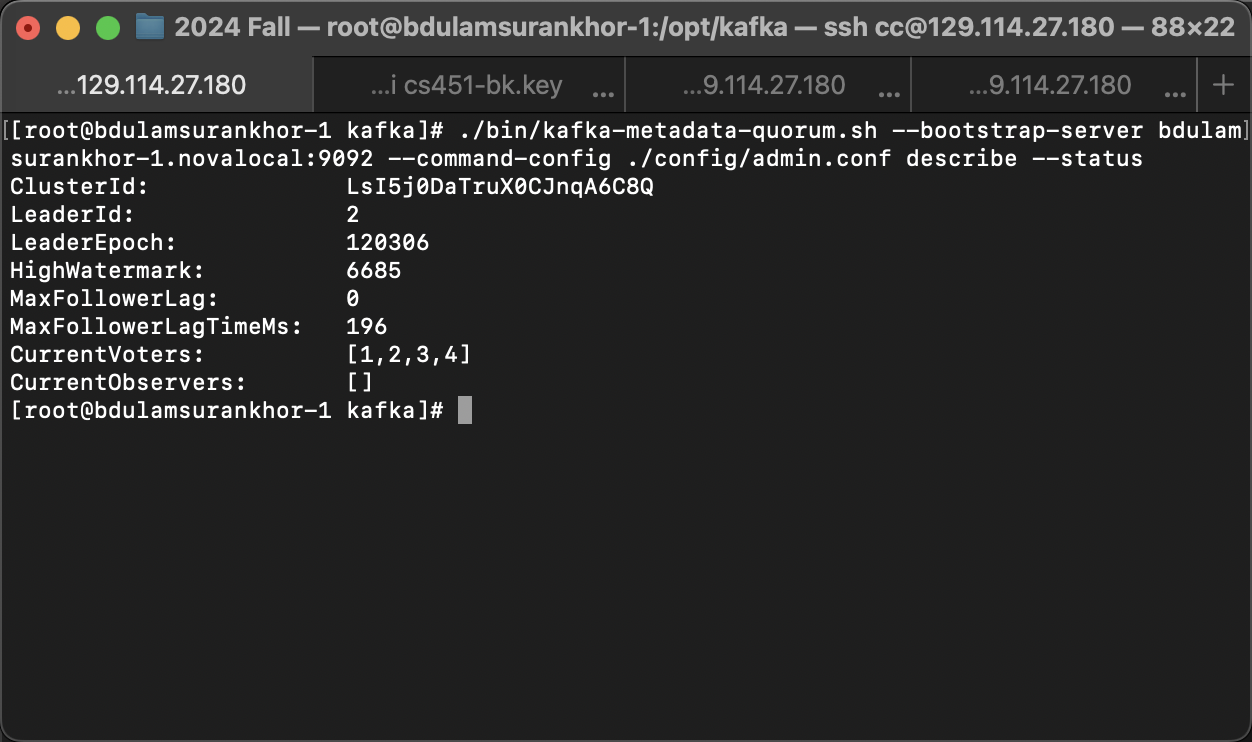
\includegraphics[width=\textwidth]{image1.png}
    \caption{Screenshot at 16.}
  \end{figure}
  \begin{figure}[H]
    \centering
    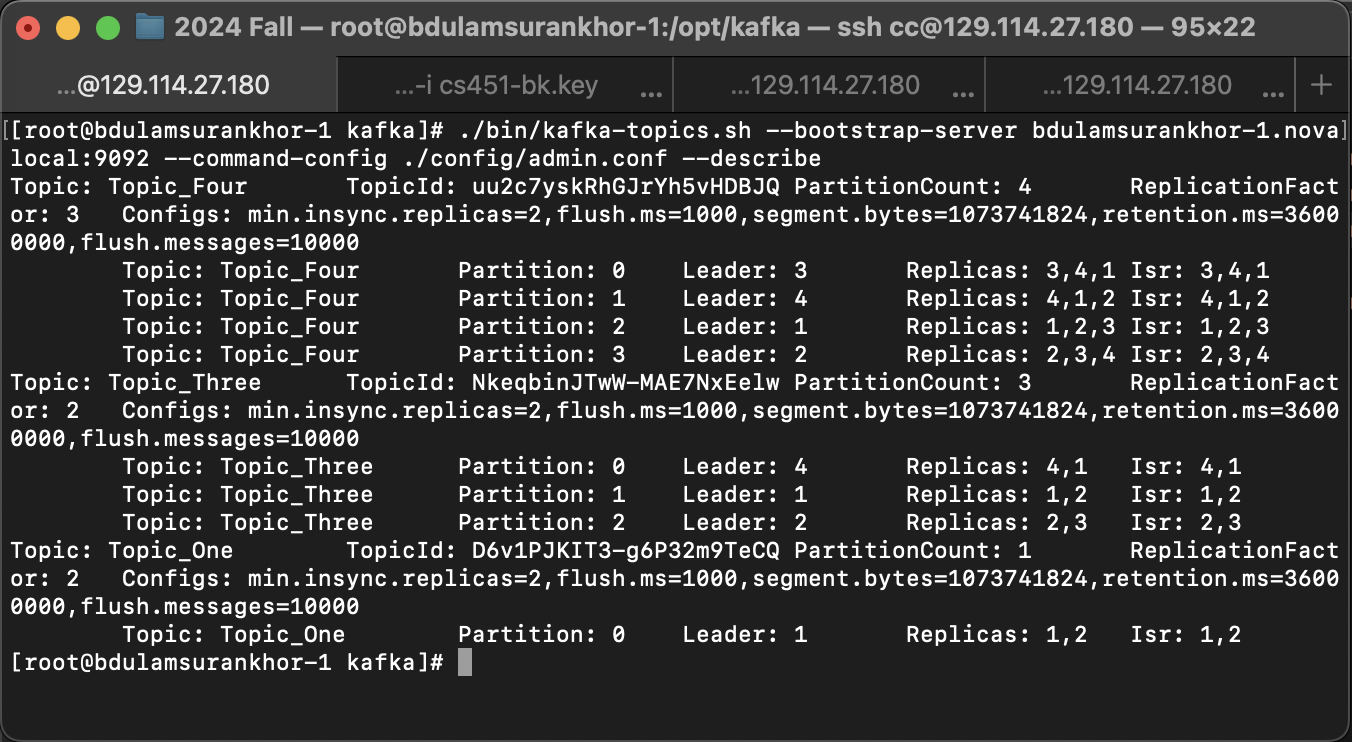
\includegraphics[width=\textwidth]{image2.png}
    \caption{Screenshot at 17.}
  \end{figure}
  \begin{figure}[H]
    \centering
    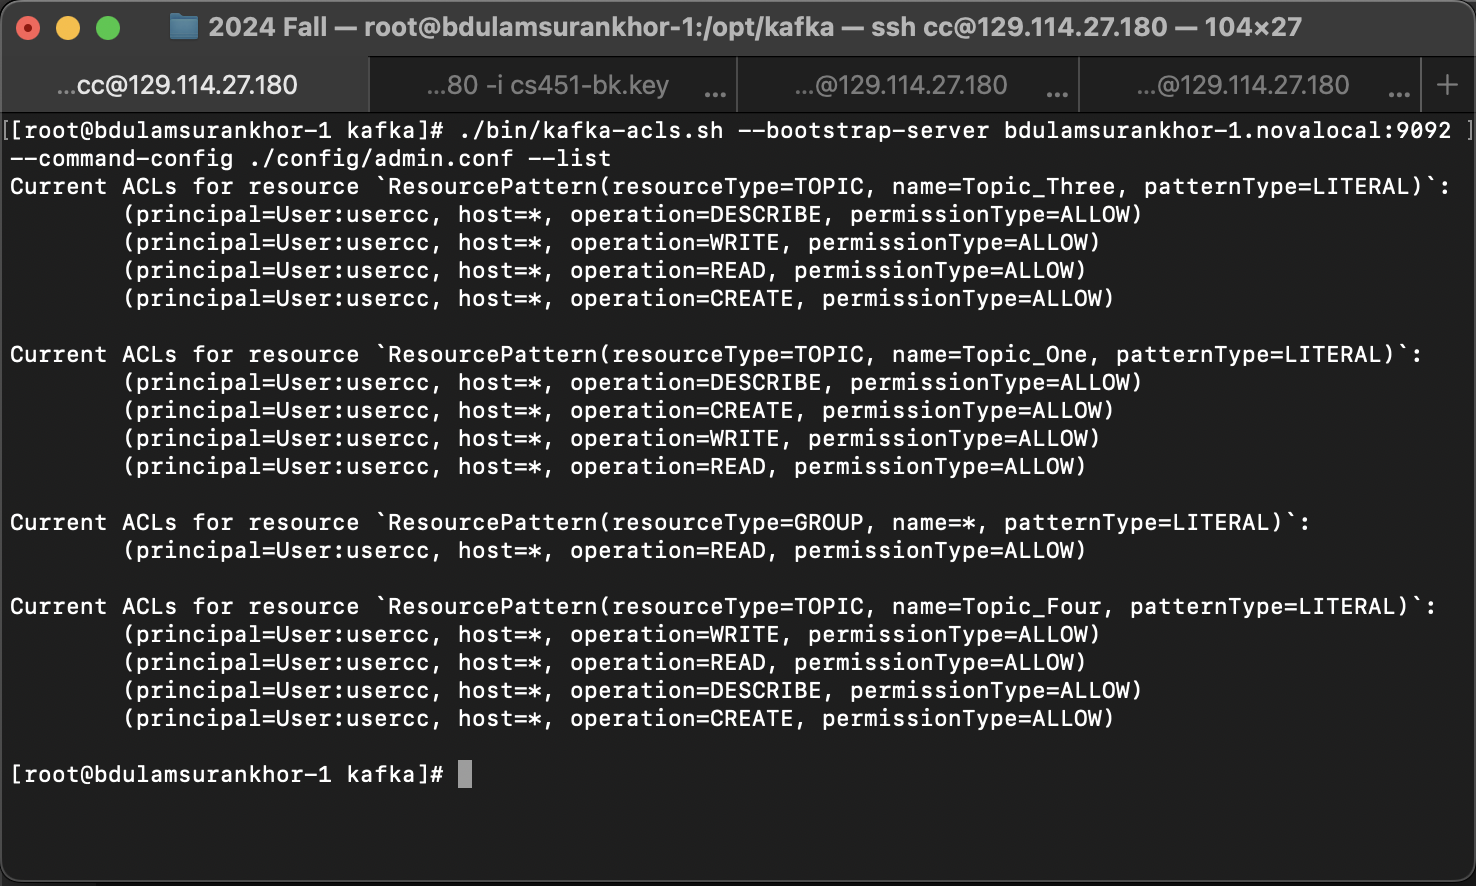
\includegraphics[width=\textwidth]{image3.png}
    \caption{Screenshot at 20.}
  \end{figure}
  \item Explain the write process when the producer wrote a message

  When the producer sends data, it first determines which partition the data is written to.
  When writing to Topic One it will be written to the only partition it has.
  Because we didn't specify key when sending message, kafka uses round-robin to distribute messages across partitions.
  The producer then sends the message to the leader for the chosen partition.
  The leader broker sends back acknowledgement to the producer.
  Kafka then replicates the message depending on the replication factor for fault tolerance.

  \item Why did we enable SSL?

  The primary reason is for security.
  By using SSL protocol, we ensure that the message we are sending between user and kafka is encrypted and authenticated.
  We sign the message with the certificate and kafka checks the signiture for authenticity, so we are able to authorize and communicate with kafka.
  Also, by encrypting the message, an intercepted message would be unreadable.

  \item Who and what is the principle?

  Principle is an identity that can be authenticated.
  In our case, it is user(producer, consumer) who is connecting to kafka brokers, or brokers who are communicating between each other.
  Examining the certificate gives:
  
  openssl x509 -in cert.crt -text -noout

        Serial Number:

            4a:4b:4b:40:c5:3e:d3:7f:f5:90:5f:fc:28:b5:5e:82:71:77:14:a2

        Signature Algorithm: sha256WithRSAEncryption

        Issuer: C = US, ST = ILLINOIS, L = CHICAGO, O = IIT, OU = CS, CN = kafka-1.novalocal, emailAddress = blenard@iit.edu

        Validity

            Not Before: Sep 25 02:23:59 2024 GMT

            Not After : Sep 23 02:23:59 2034 GMT

        Subject: C = US, ST = ILLINOIS, L = CHICAGO, O = IIT, OU = CS, CN = kafka-1.novalocal, emailAddress = blenard@iit.edu

  \item Shutdown 1 of the 4 nodes, try reading and writing messages like in part 2. What happened to which topic? (sudo systemctl stop kafka)

  Topic One and Topic Three fails when writing a message. The error says NOT ENOUGH REPLICAS.

  \begin{figure}[H]
    \centering
    \begin{minipage}{0.45\textwidth}
      \centering
      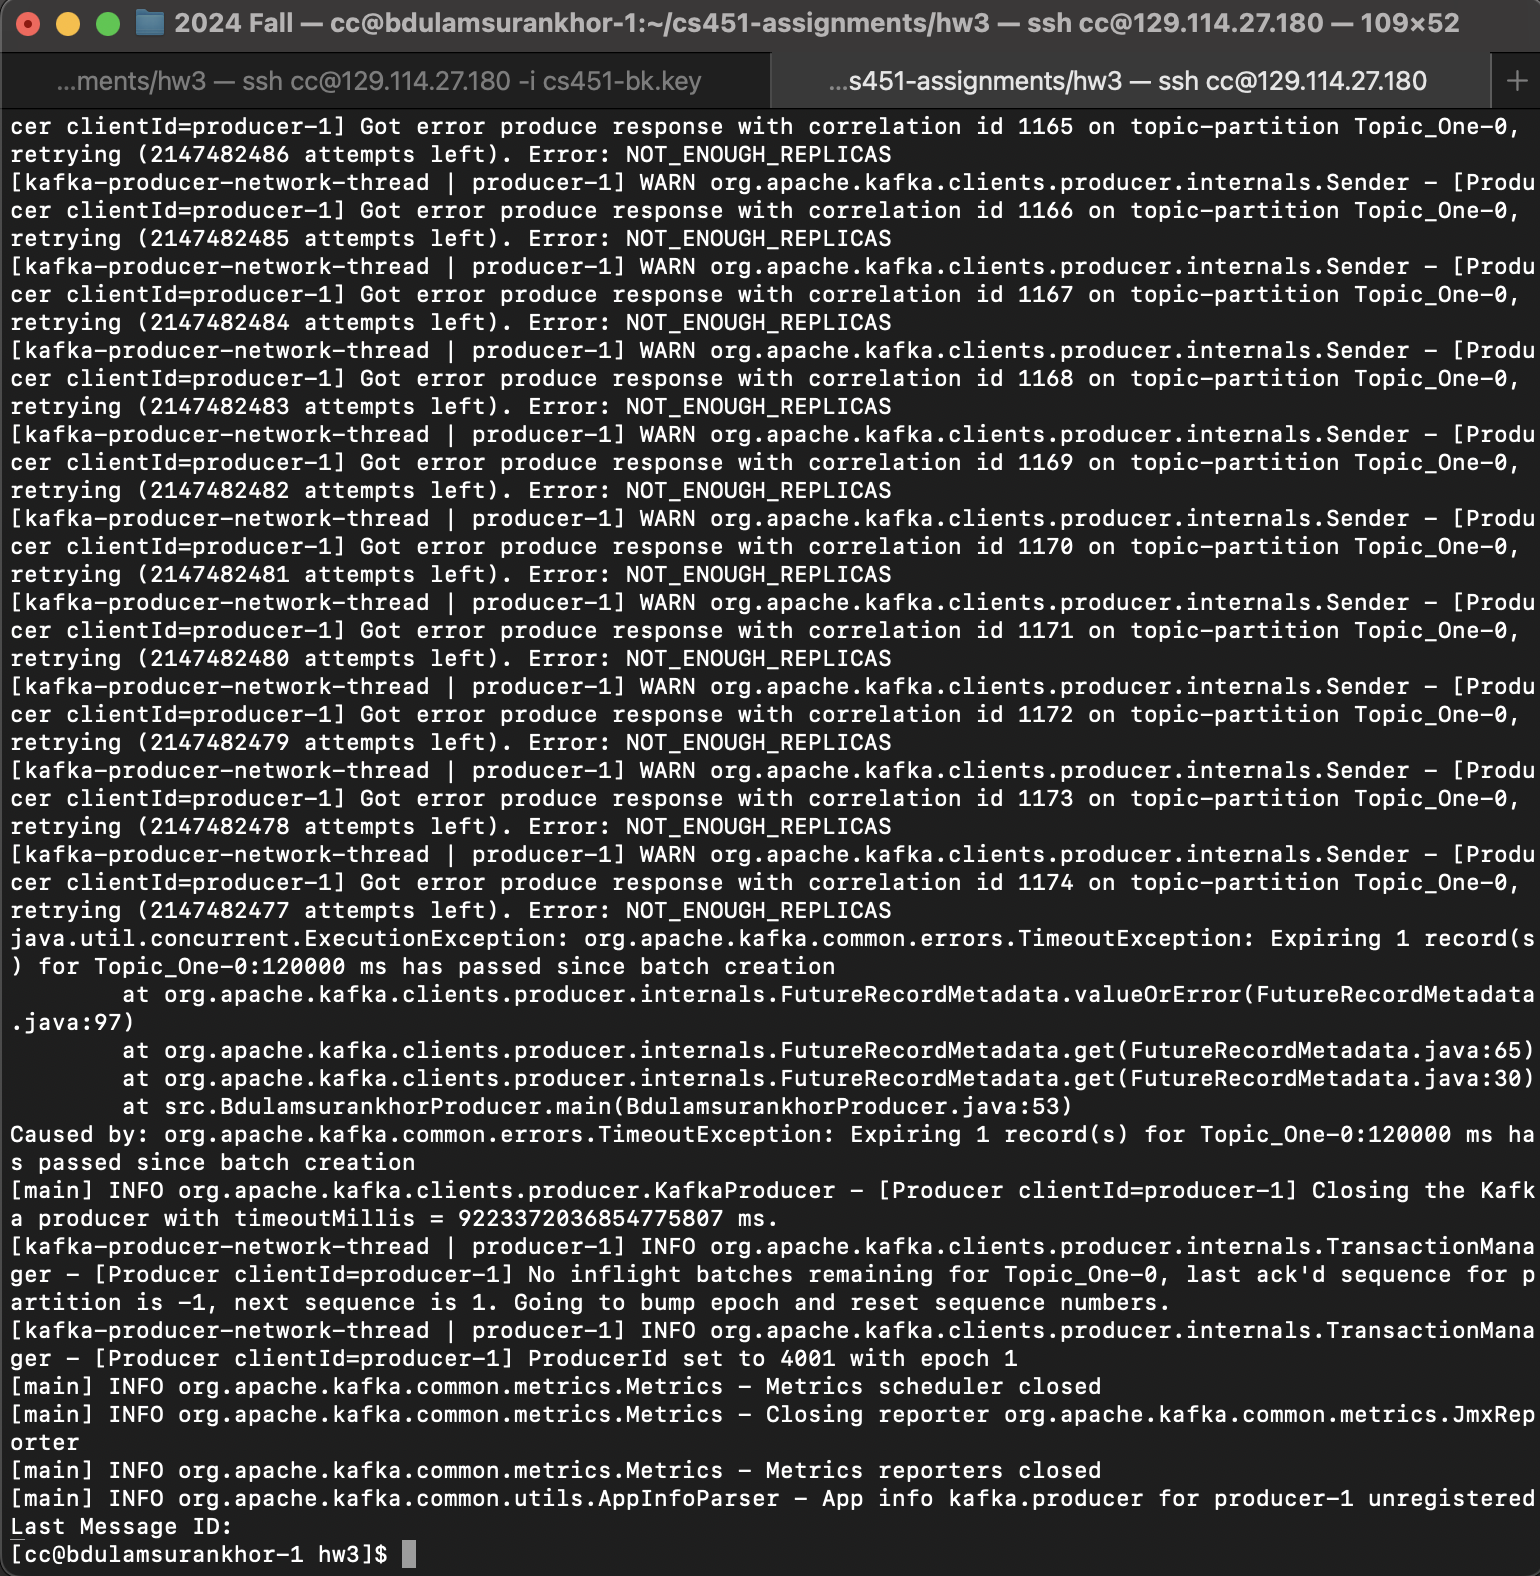
\includegraphics[width=1\textwidth]{image4.png}
      \caption{Topic\_One output after shutting down 1 node.}
    \end{minipage}
    \begin{minipage}{0.45\textwidth}
      \centering
      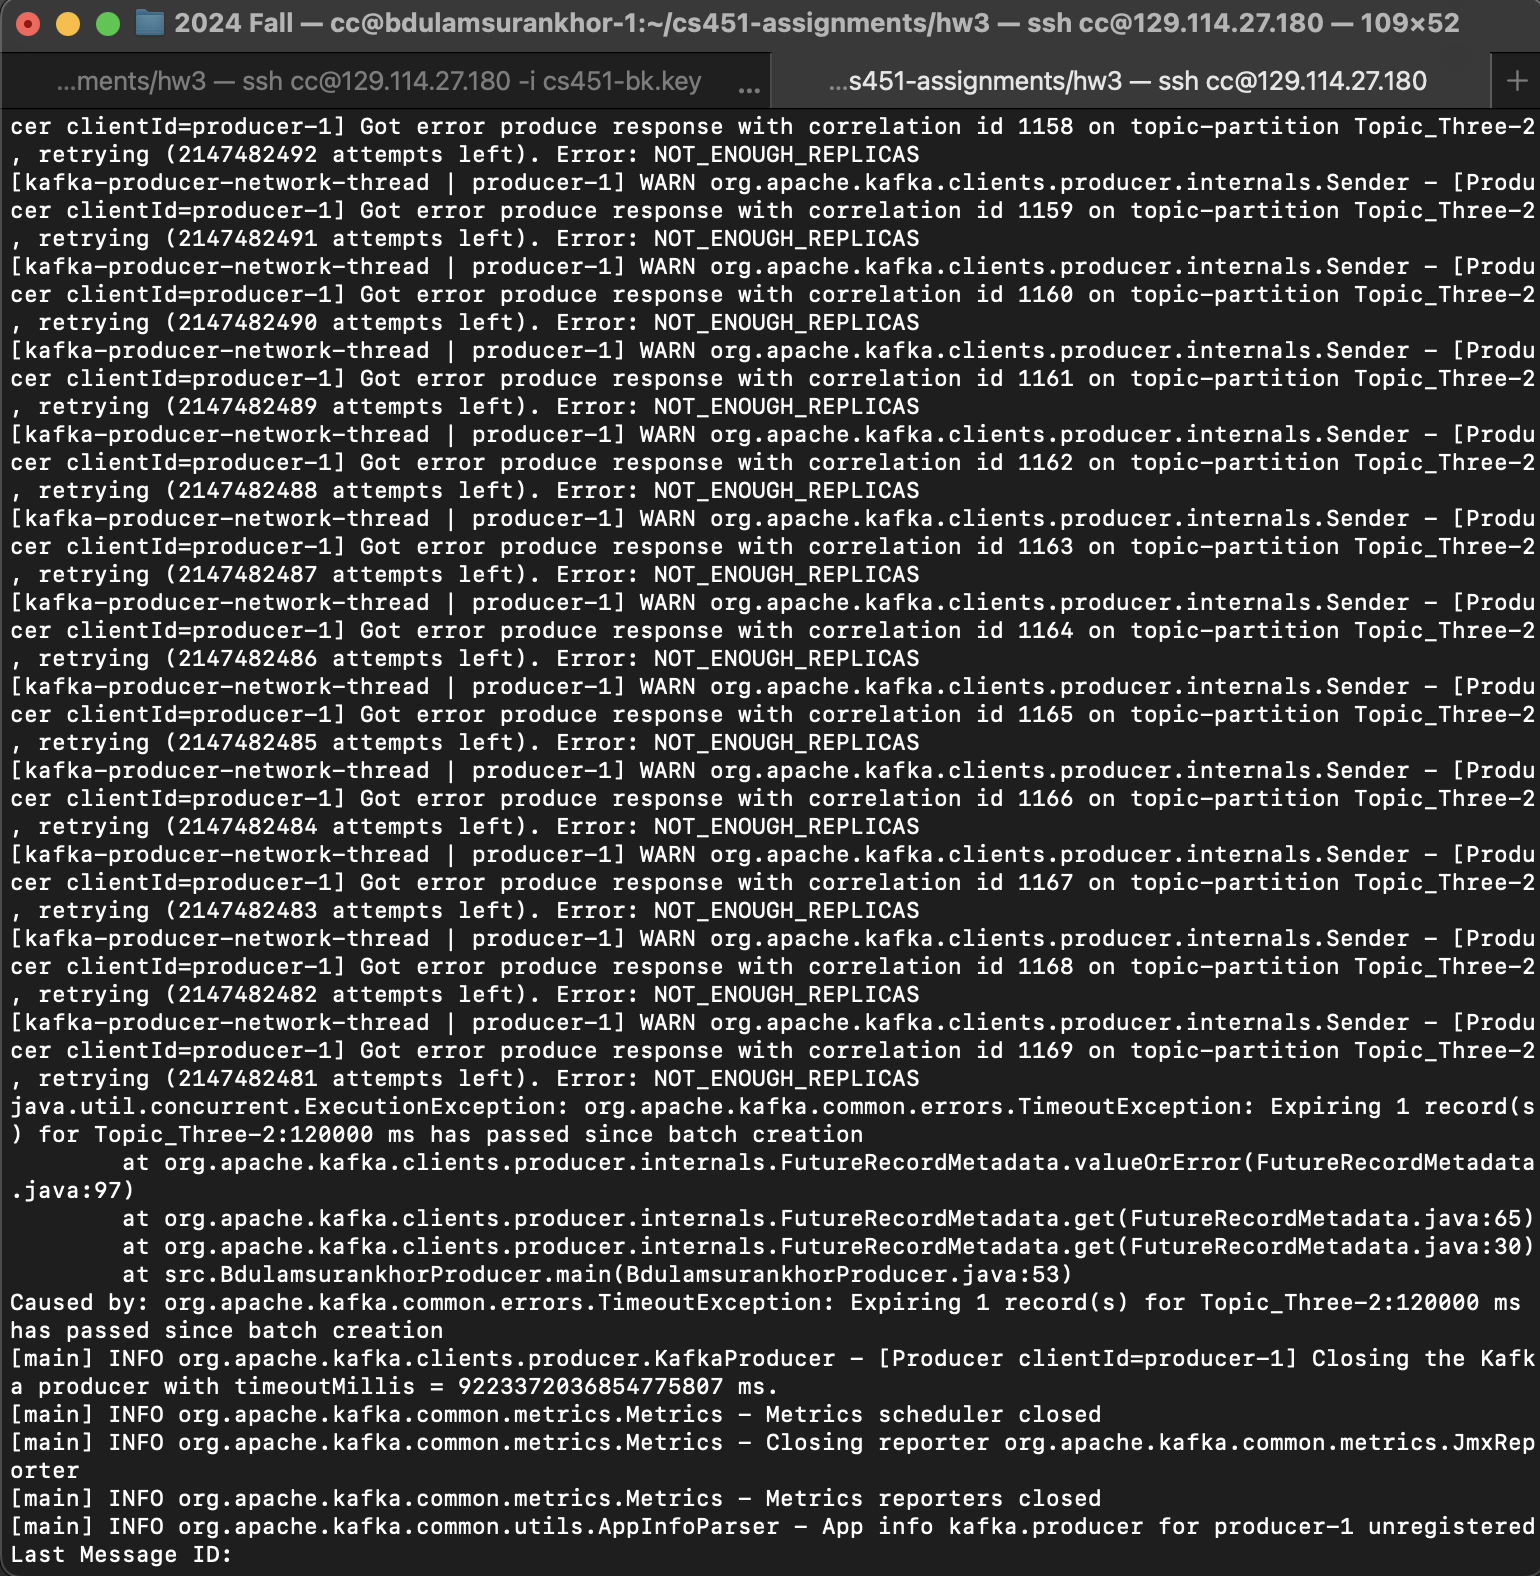
\includegraphics[width=1\textwidth]{image5.png}
      \caption{Topic\_Three output after shutting down 1 node.}
    \end{minipage}
  \end{figure}

  Topic Four writes and writes successfully like on step 2.

  \begin{figure}[H]
    \centering
    \begin{minipage}{0.45\textwidth}
      \centering
      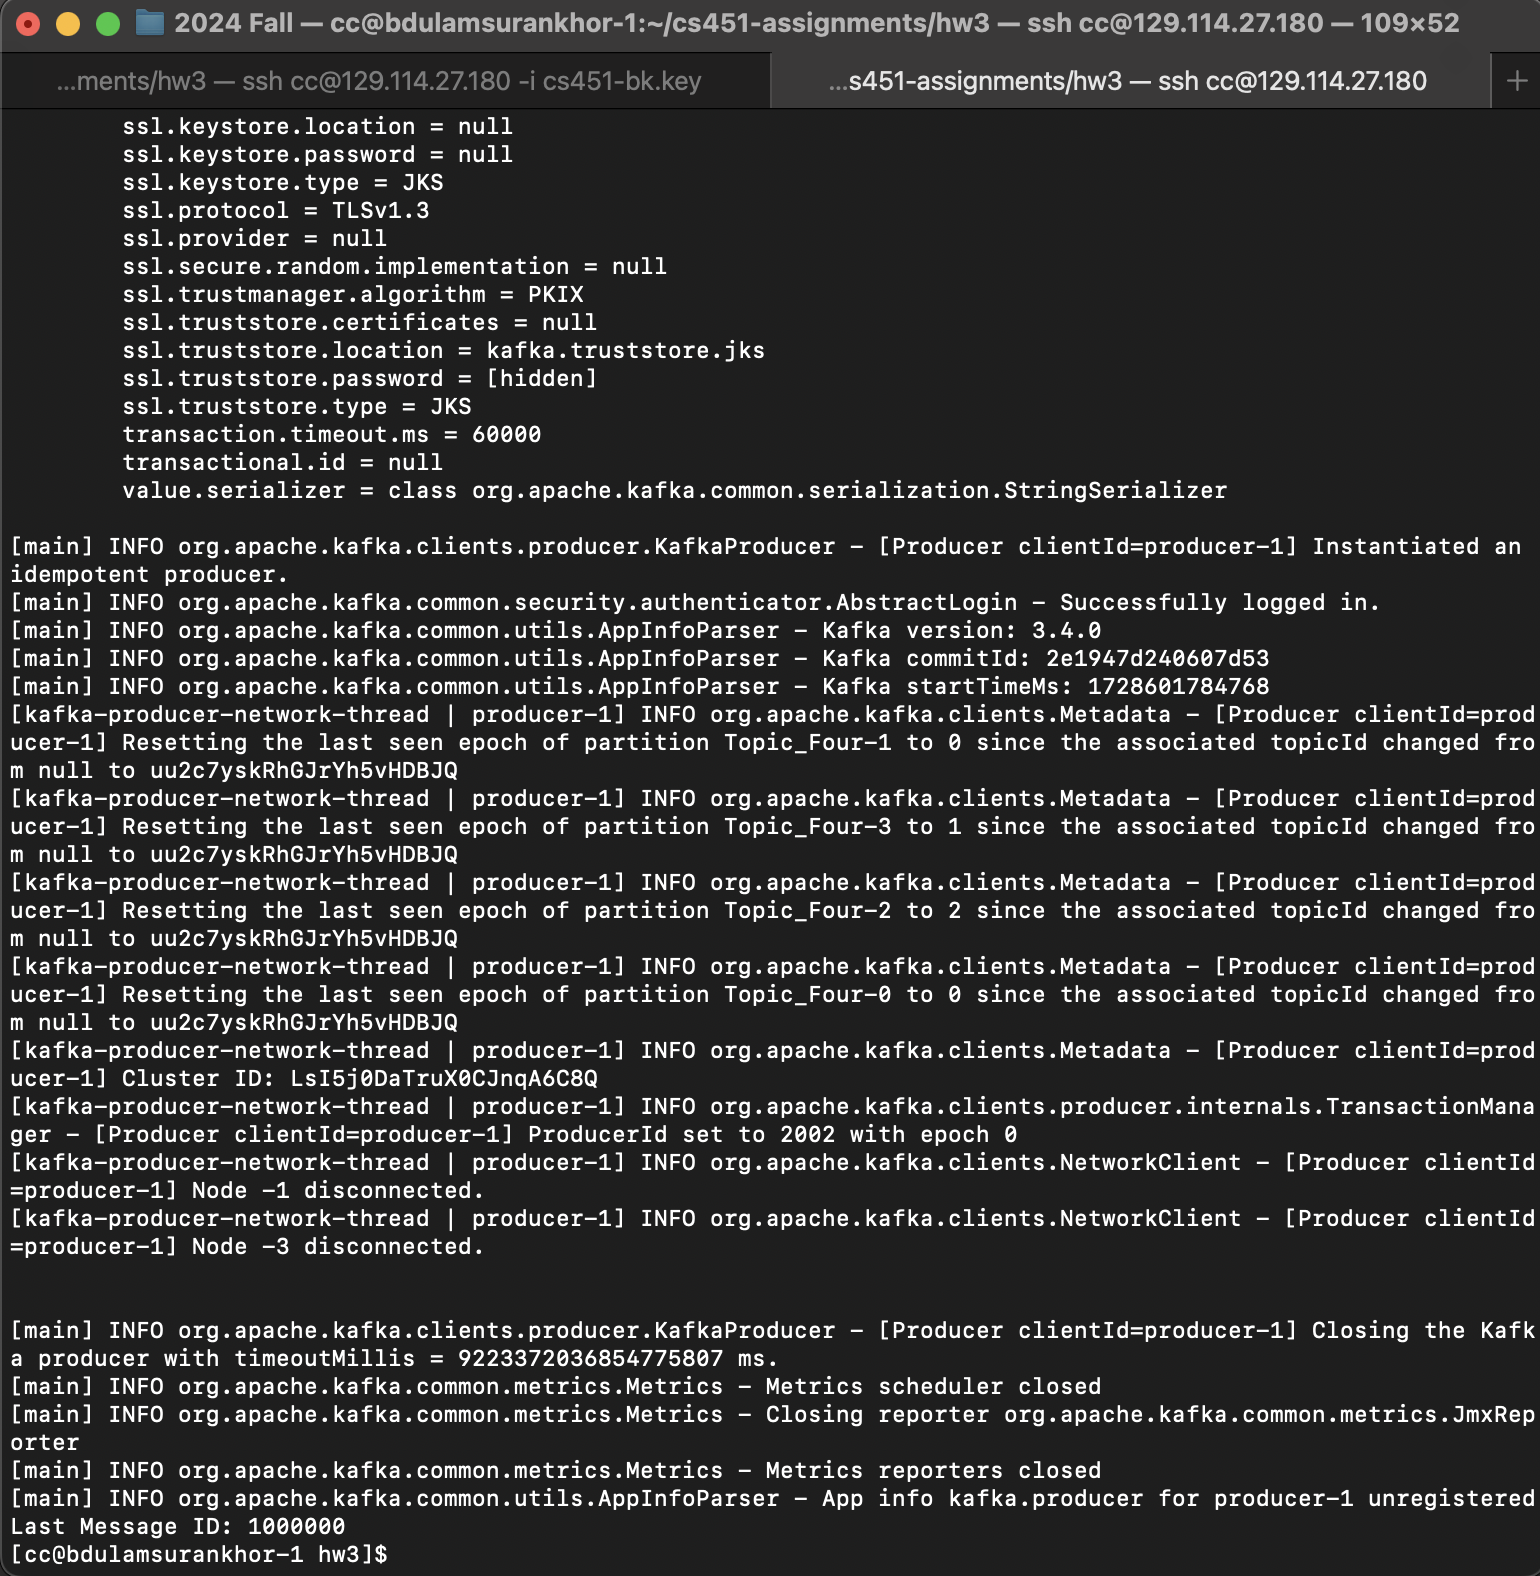
\includegraphics[width=1\textwidth]{image6.png}
      \caption{Topic\_Four producer output after shutting down 1 node.}
    \end{minipage}
    \begin{minipage}{0.45\textwidth}
      \centering
      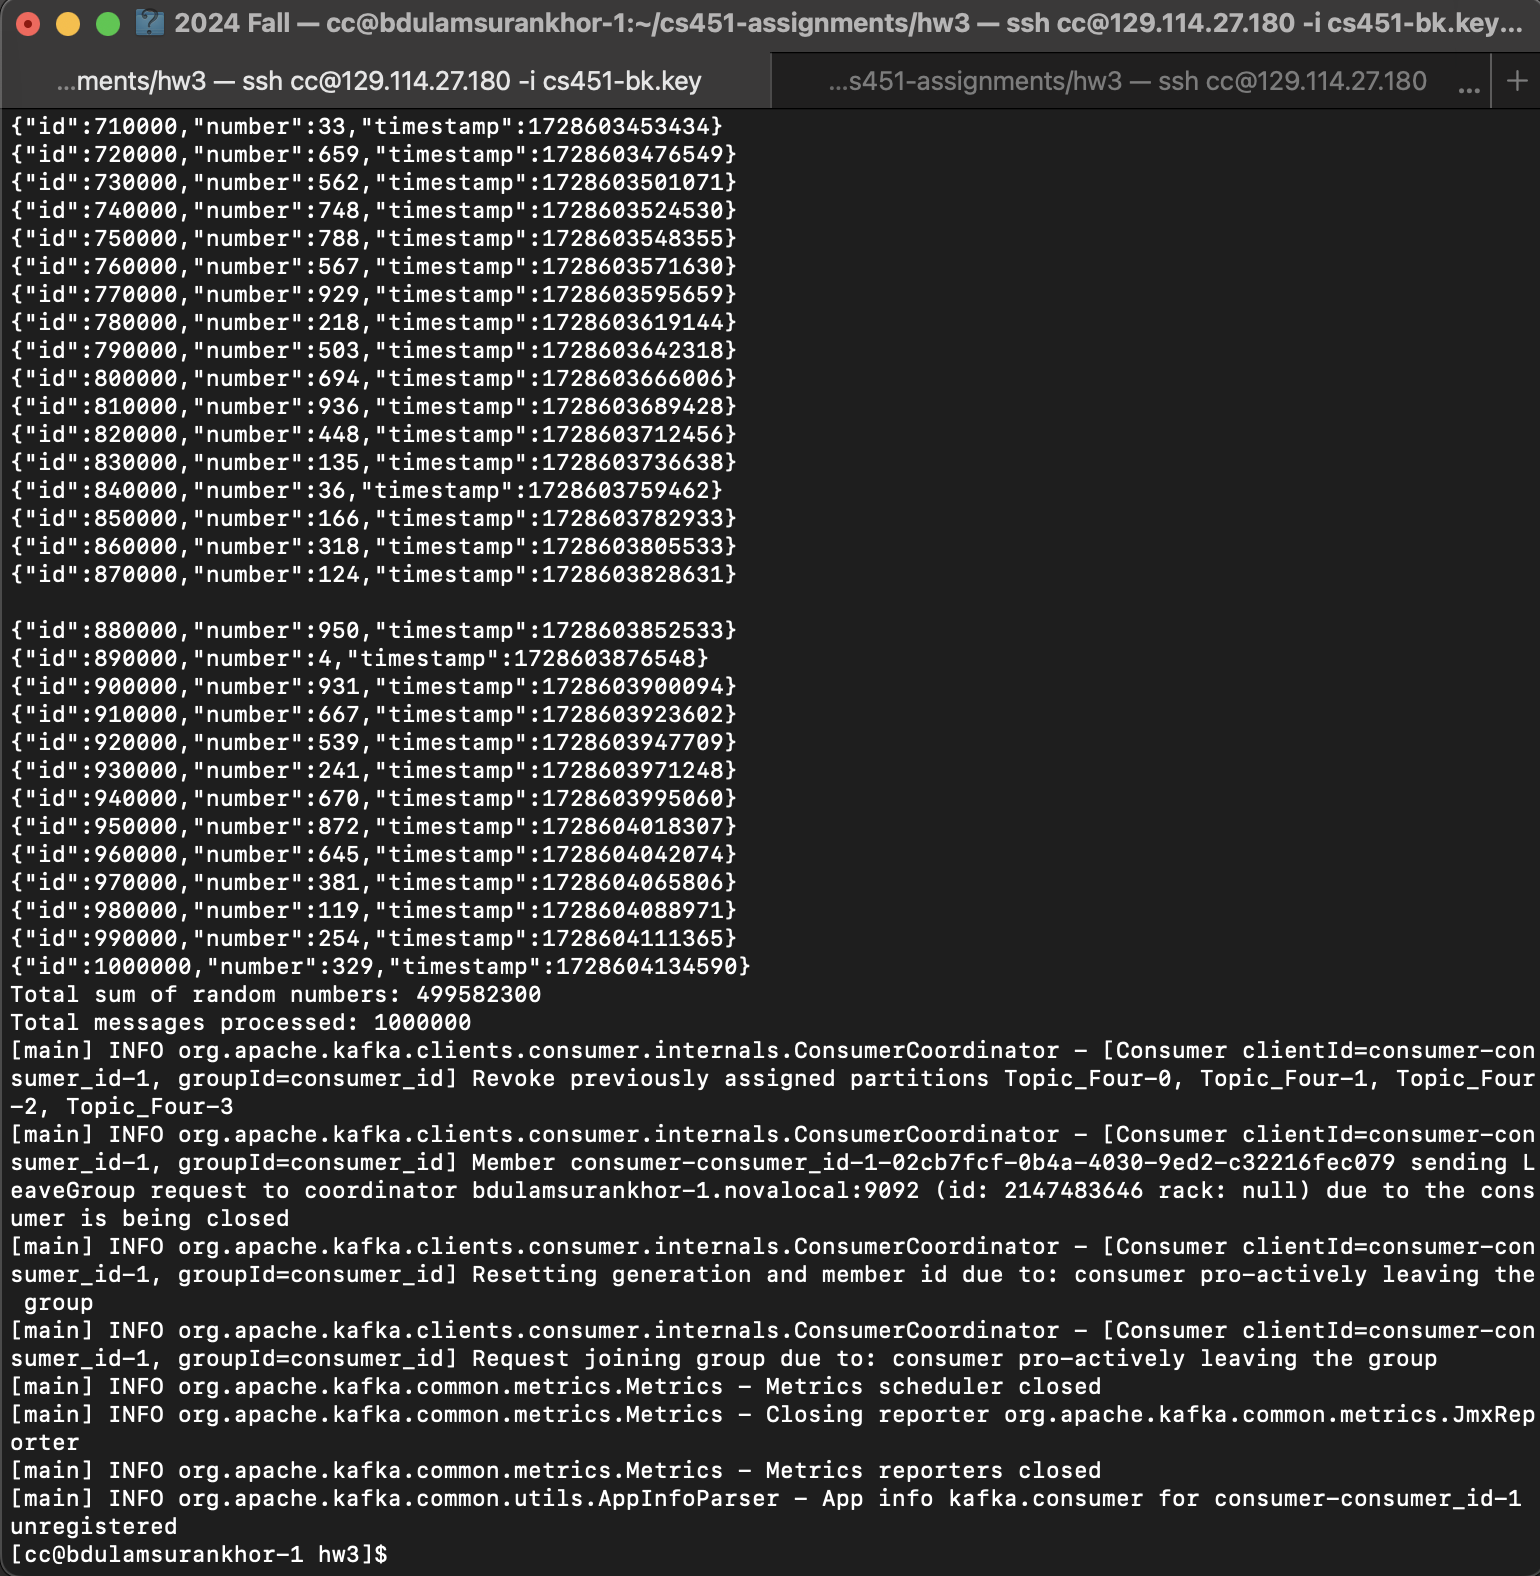
\includegraphics[width=1\textwidth]{image7.png}
      \caption{Topic\_Four consumer output after shutting down 1 node.}
    \end{minipage}
  \end{figure}

  \item Shutdown 2 of the 4 nodes, try reading and writing messages like in part 2. What happened to which topic? (sudo systemctl stop kafka)

  This time, producer fails to write to all three topics.

  \begin{figure}[H]
    \centering
    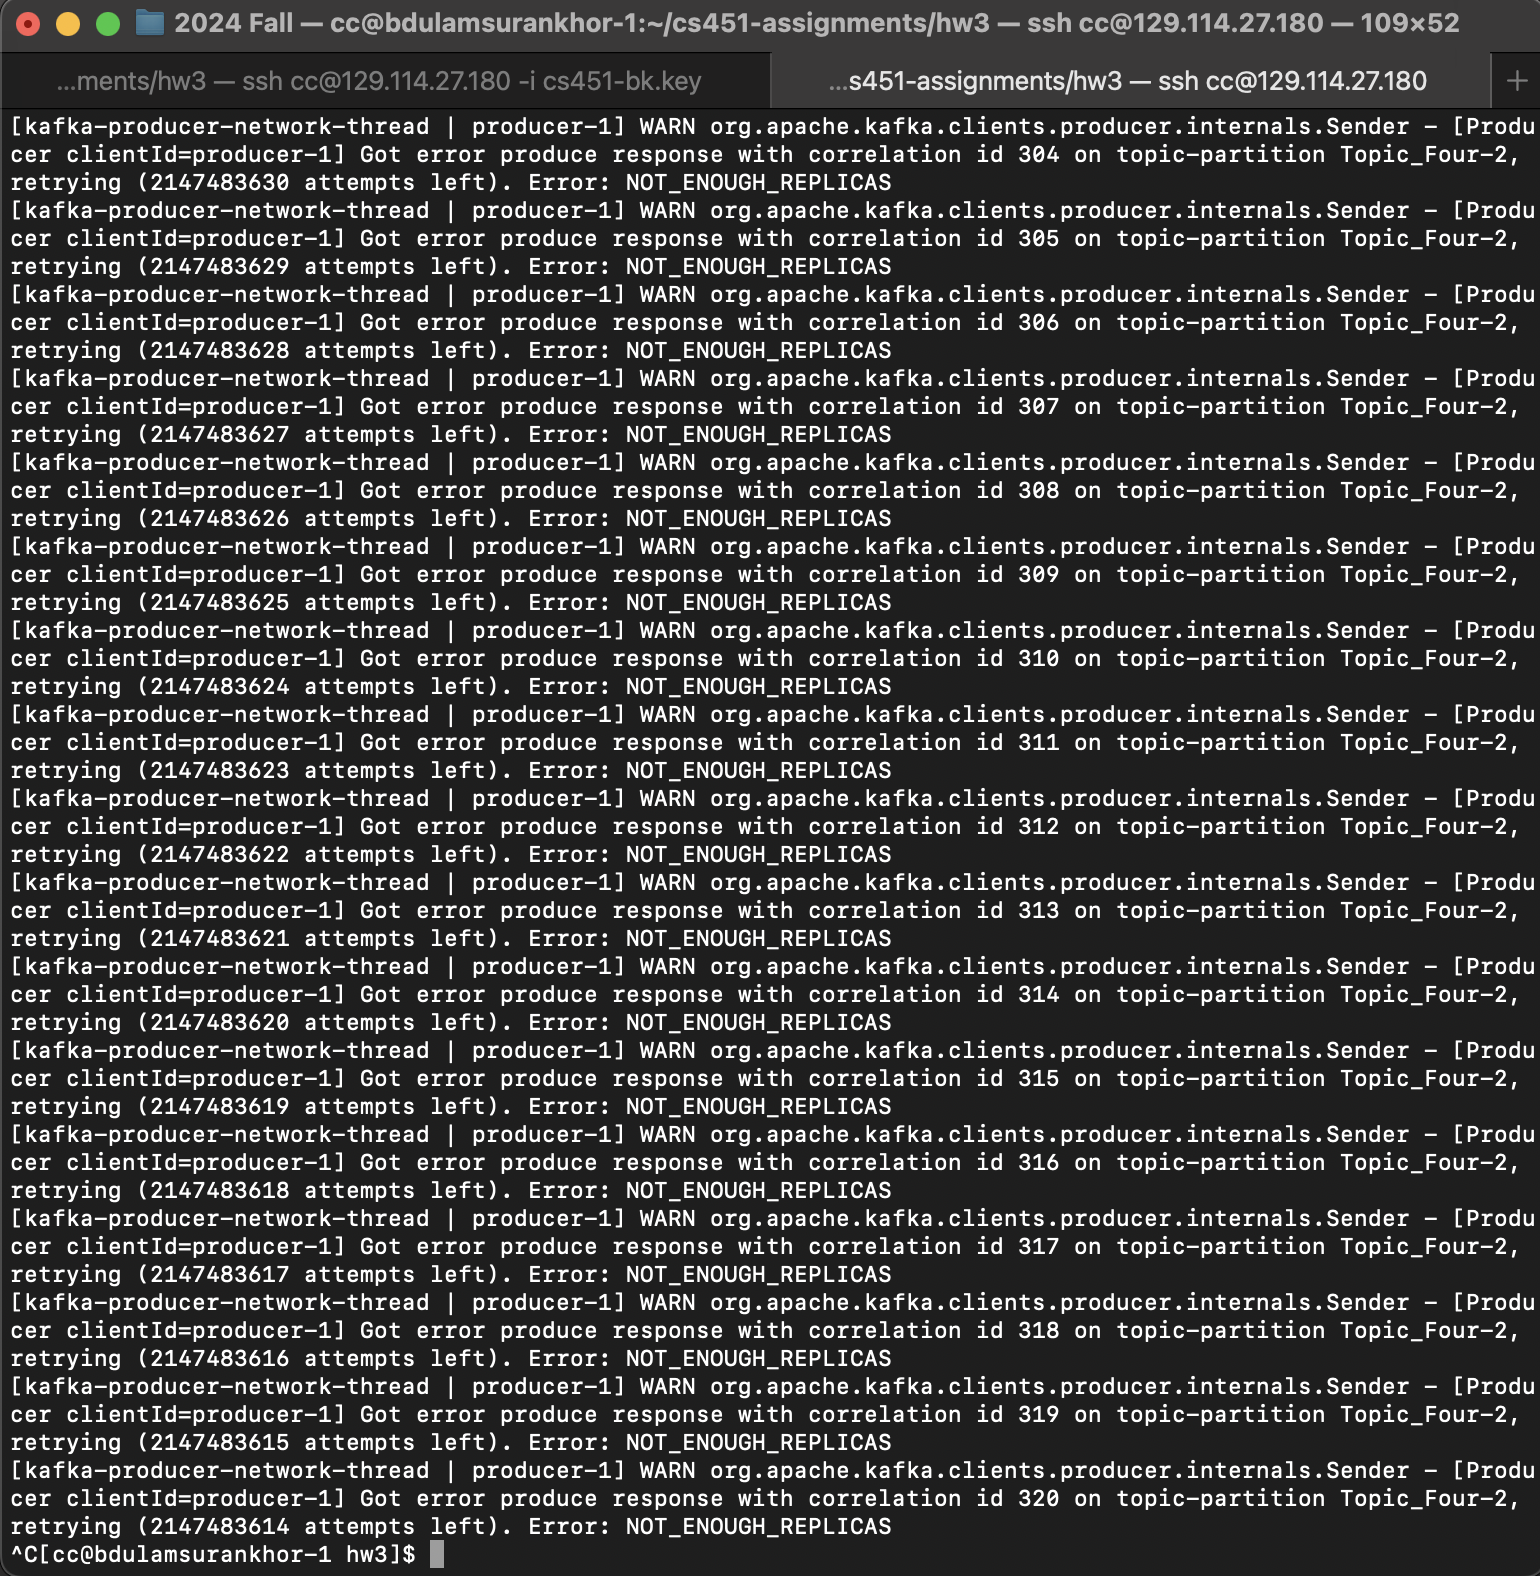
\includegraphics[width=0.45\textwidth]{image8.png}
    \caption{Topic\_Four producer output after shutting down 2 nodes.}
  \end{figure}

  \item Start the two back up (sudo systemctl start kafka) on both
  \item Rerun 17.d, are the partitions insync? Take a screenshot

  They are in sync.

  \begin{figure}[H]
    \centering
    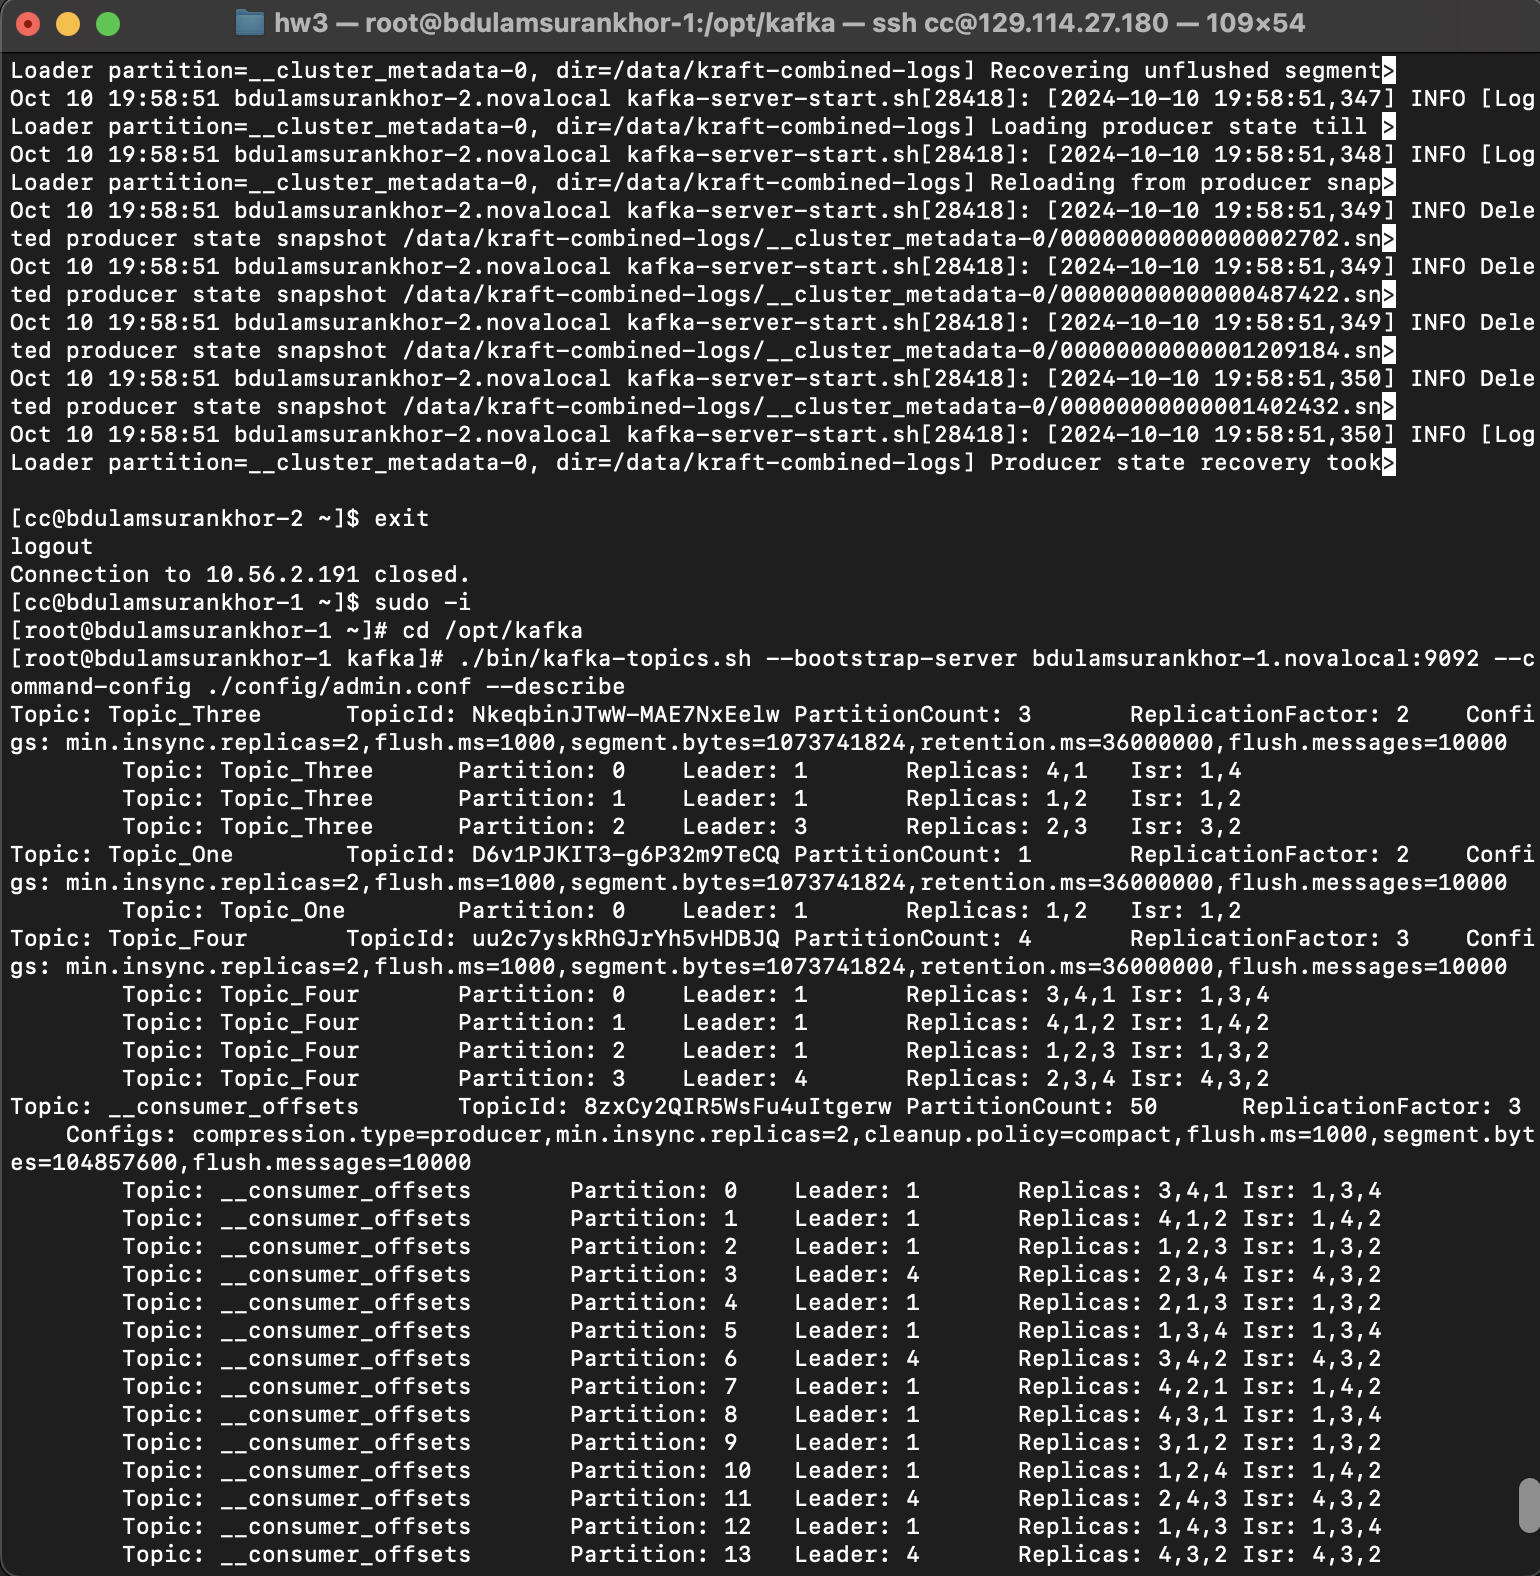
\includegraphics[width=0.45\textwidth]{image9.png}
    \caption{Screenshot after starting two brokers that previously been shutdown.}
  \end{figure}

  \item Why is kafka running as the user kafka and not root?

  The main reason is limiting the user's privileges and security.
  Kafka user should only have the permission necessary to run the application.
  Also, by dedicating a user, we can isolate kafka only processes and files.

  \vspace{1cm}

  \item Here I am including screenshots from Step two.
  On consumer, I have written print statement for every 10000 steps to make sure the process is running(shows on console screenshots).
  I also generated random numbers from 1 to 1000.

  \begin{enumerate}
    \item Topic\_One
    \begin{figure}[H]
      \centering
      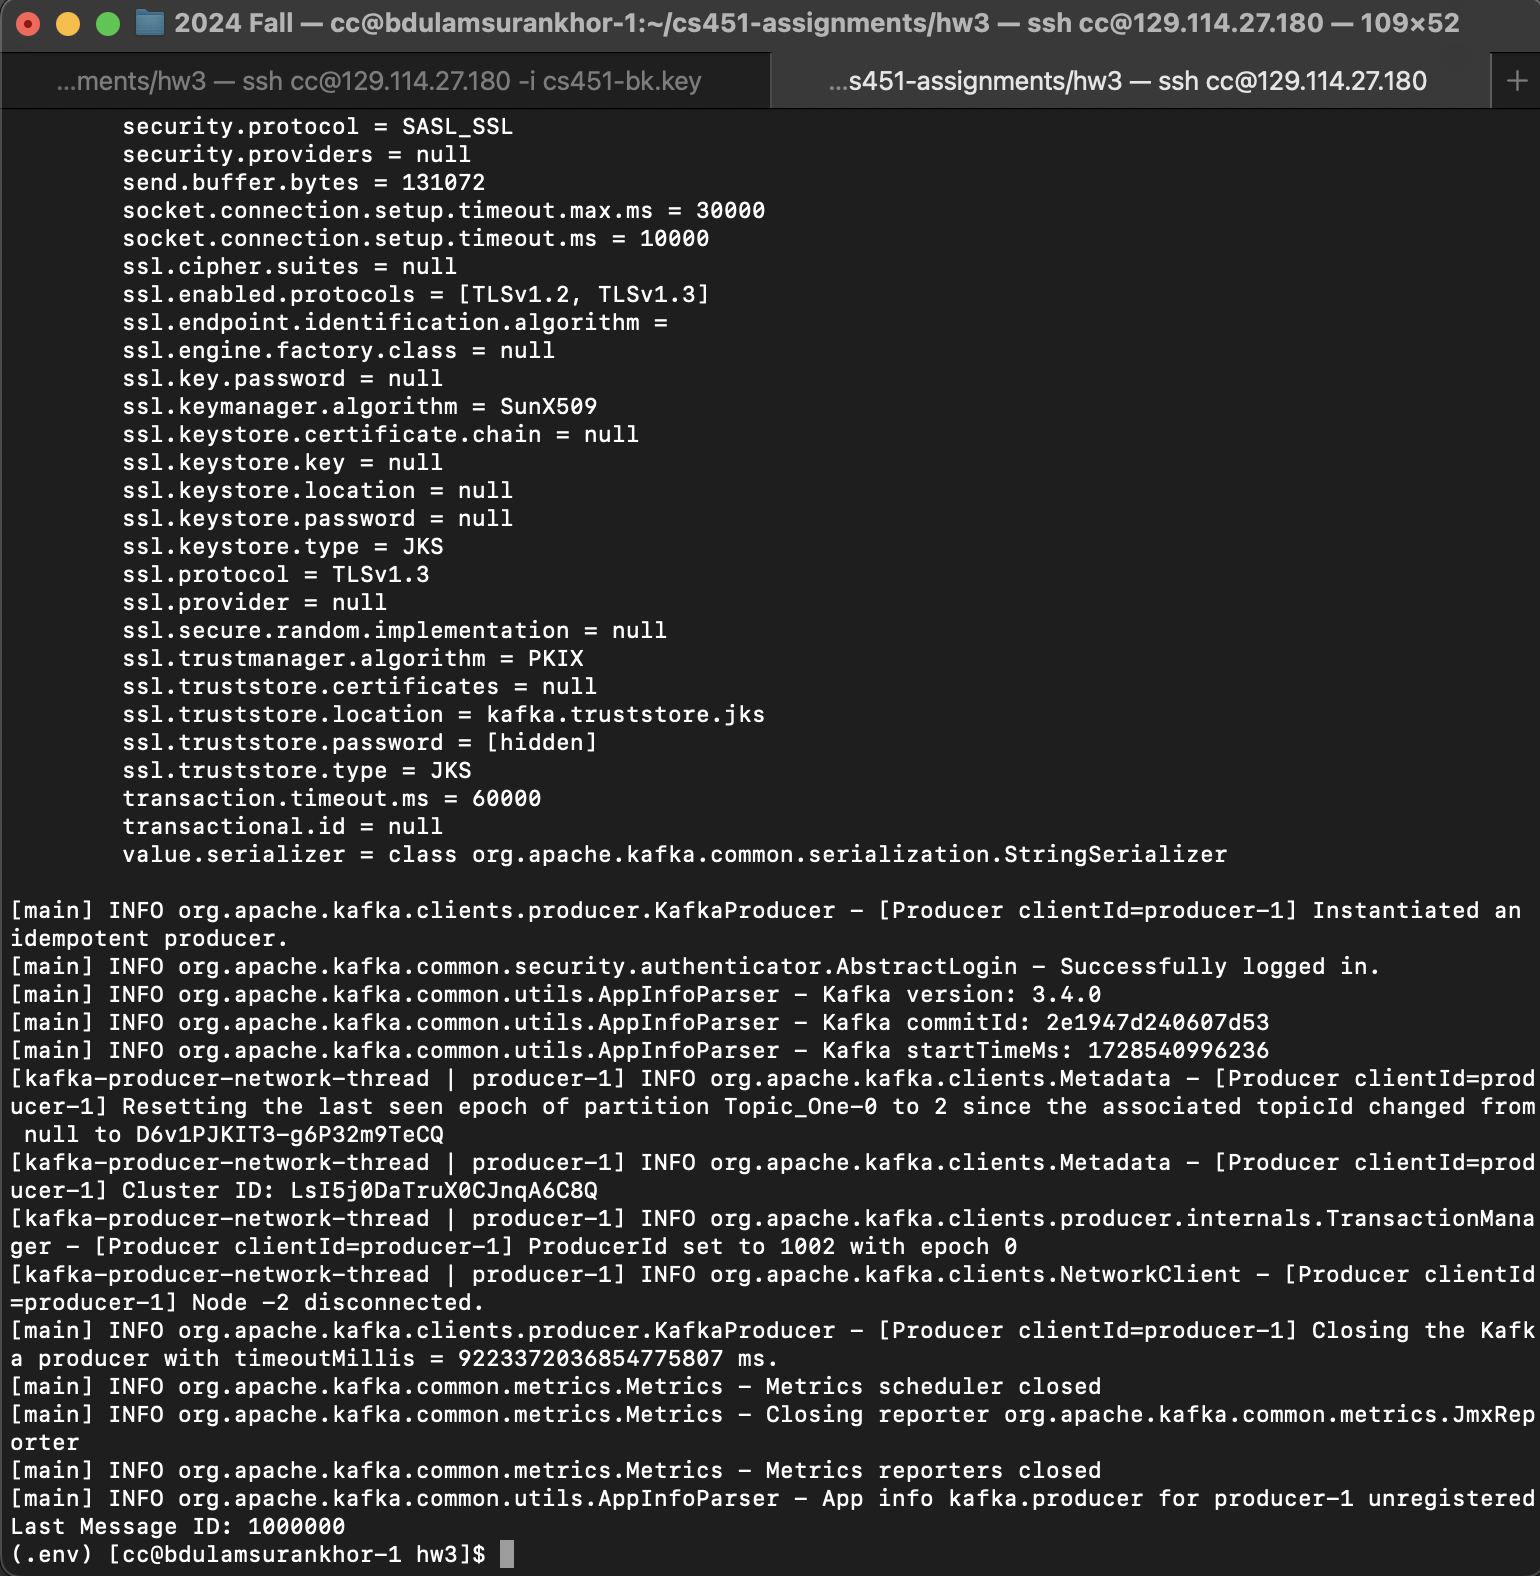
\includegraphics[width=0.6\textwidth]{image10.png}
      \caption{Topic\_One producer output.}
    \end{figure}

    \begin{figure}[H]
      \centering
      \begin{minipage}{0.45\textwidth}
        \centering
        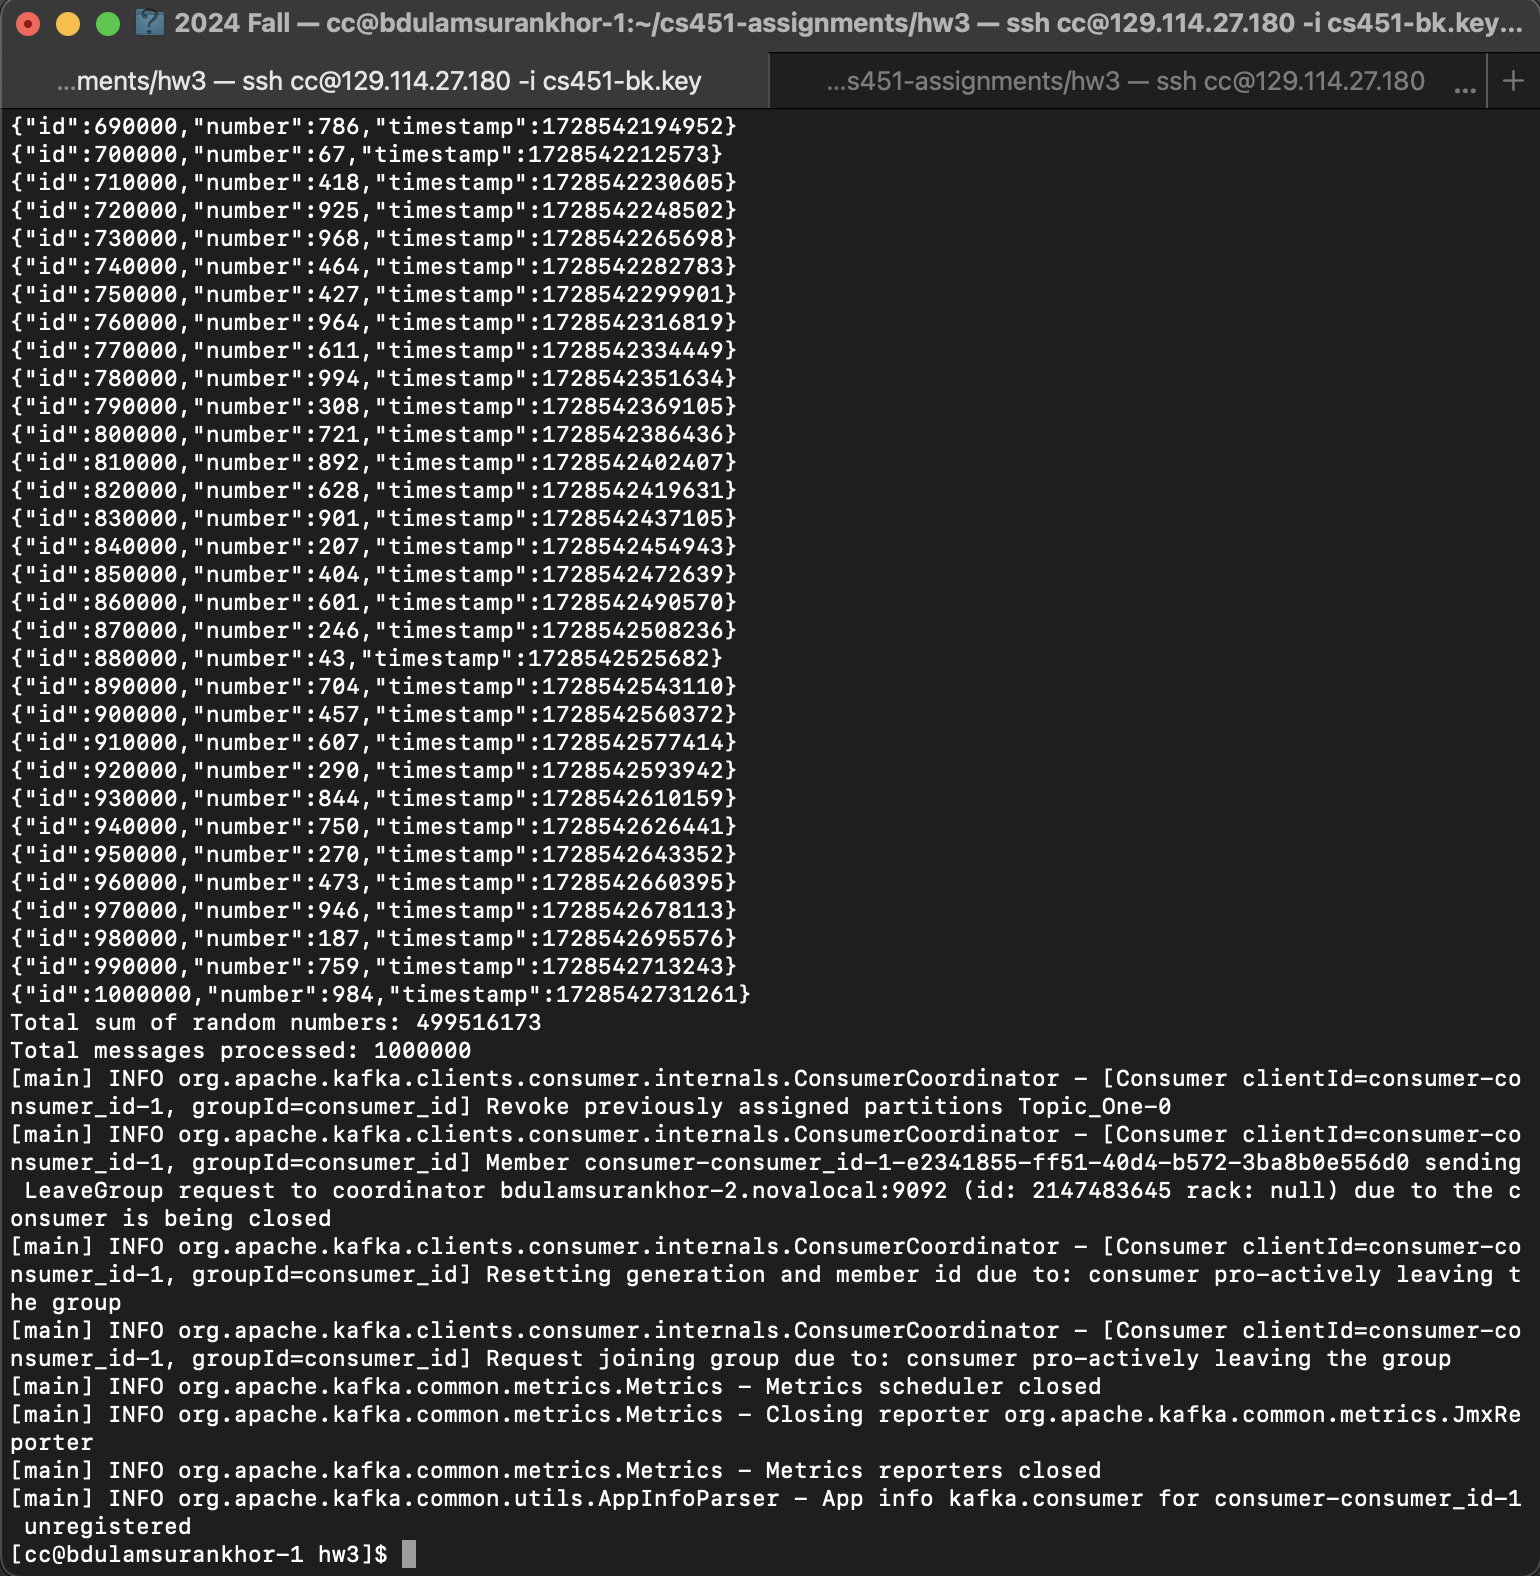
\includegraphics[width=1\textwidth]{image11.png}
        \caption{Topic\_One consumer output.}
      \end{minipage}
      \begin{minipage}{0.45\textwidth}
        \centering
        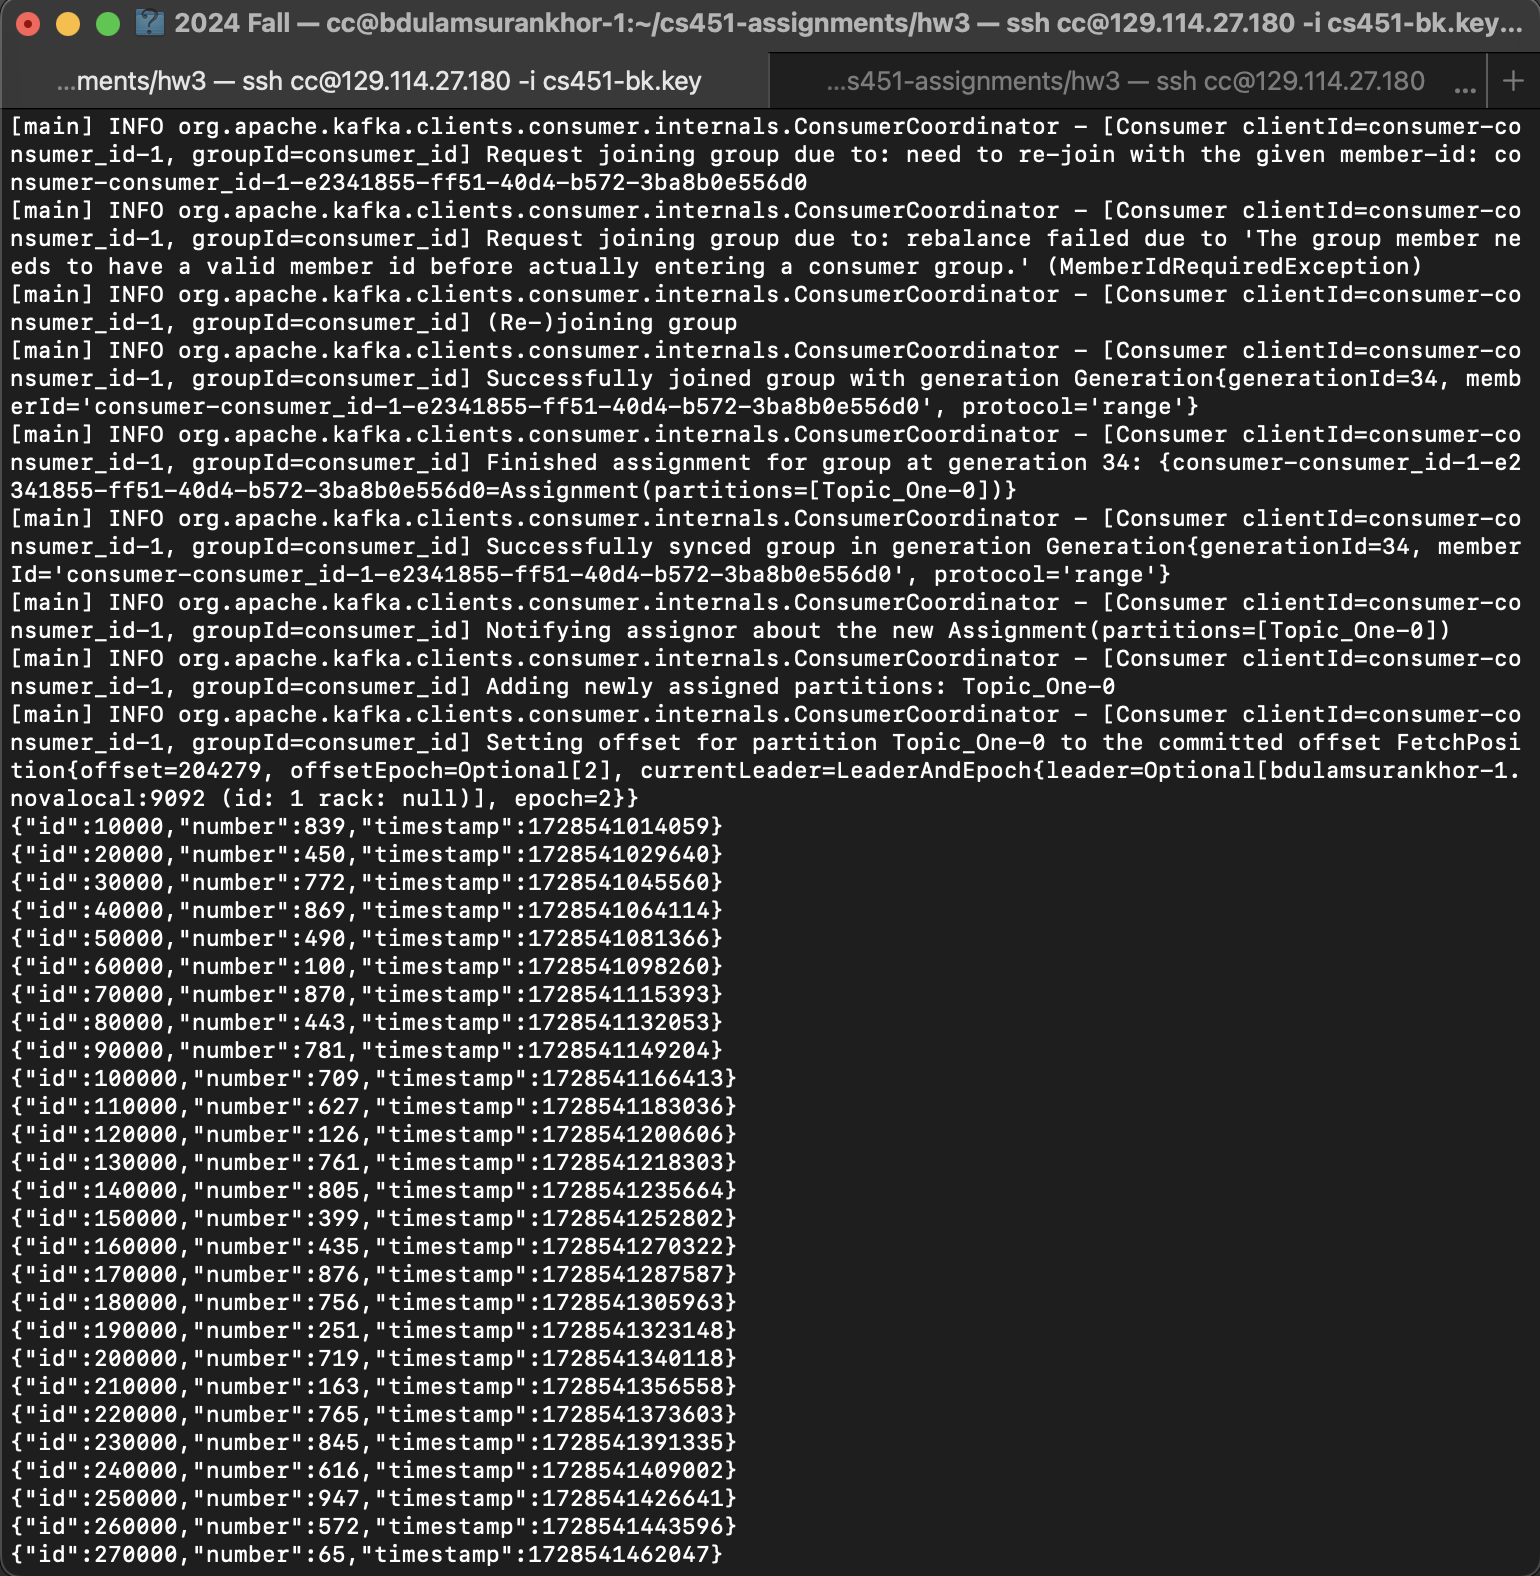
\includegraphics[width=1\textwidth]{image12.png}
        \caption{Topic\_One consumer output.}
      \end{minipage}
    \end{figure}
    \item Topic\_Three
    \begin{figure}[H]
      \centering
      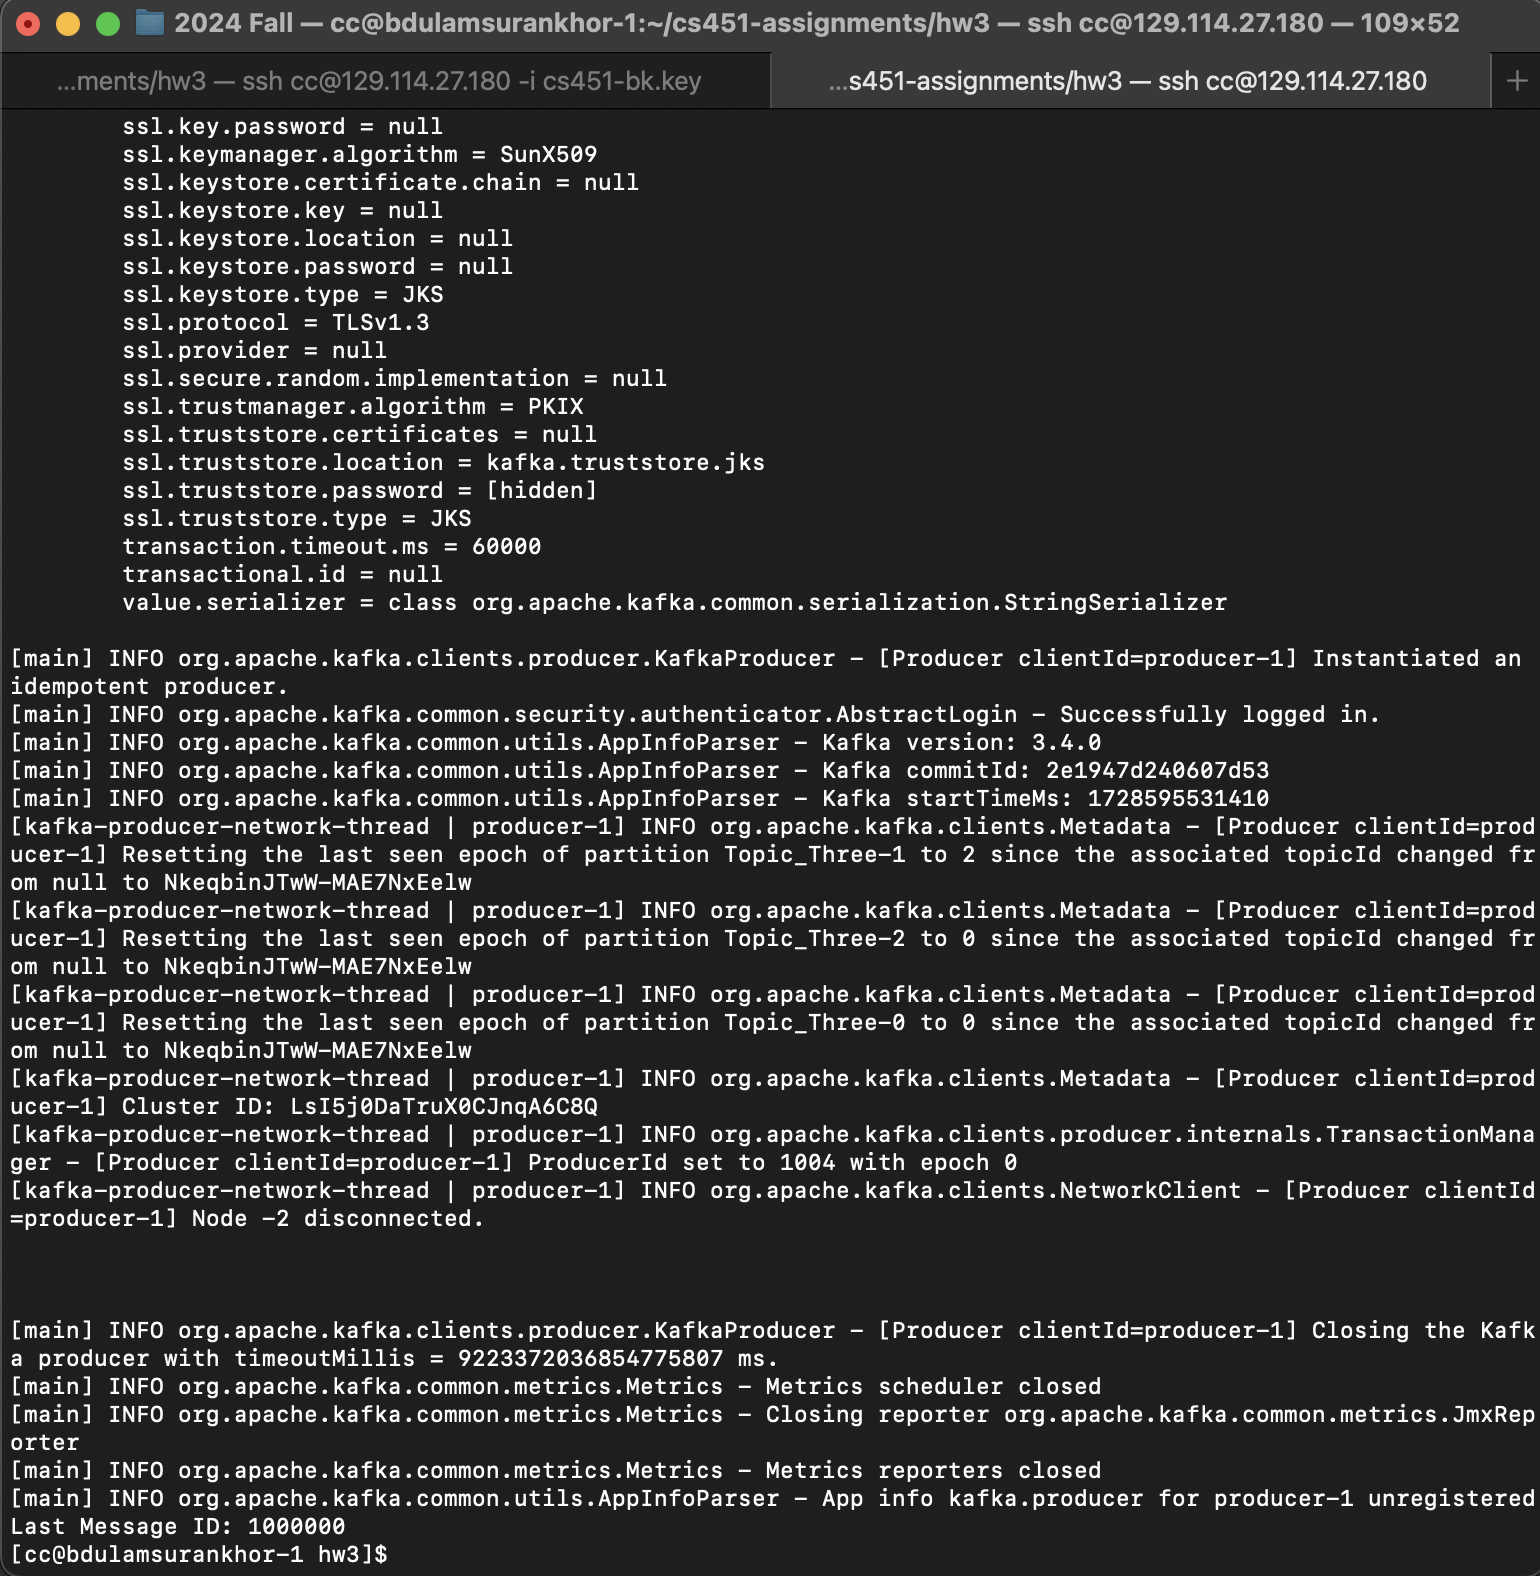
\includegraphics[width=0.6\textwidth]{image13.png}
      \caption{Topic\_Three producer output.}
    \end{figure}

    \begin{figure}[H]
      \centering
      \begin{minipage}{0.45\textwidth}
        \centering
        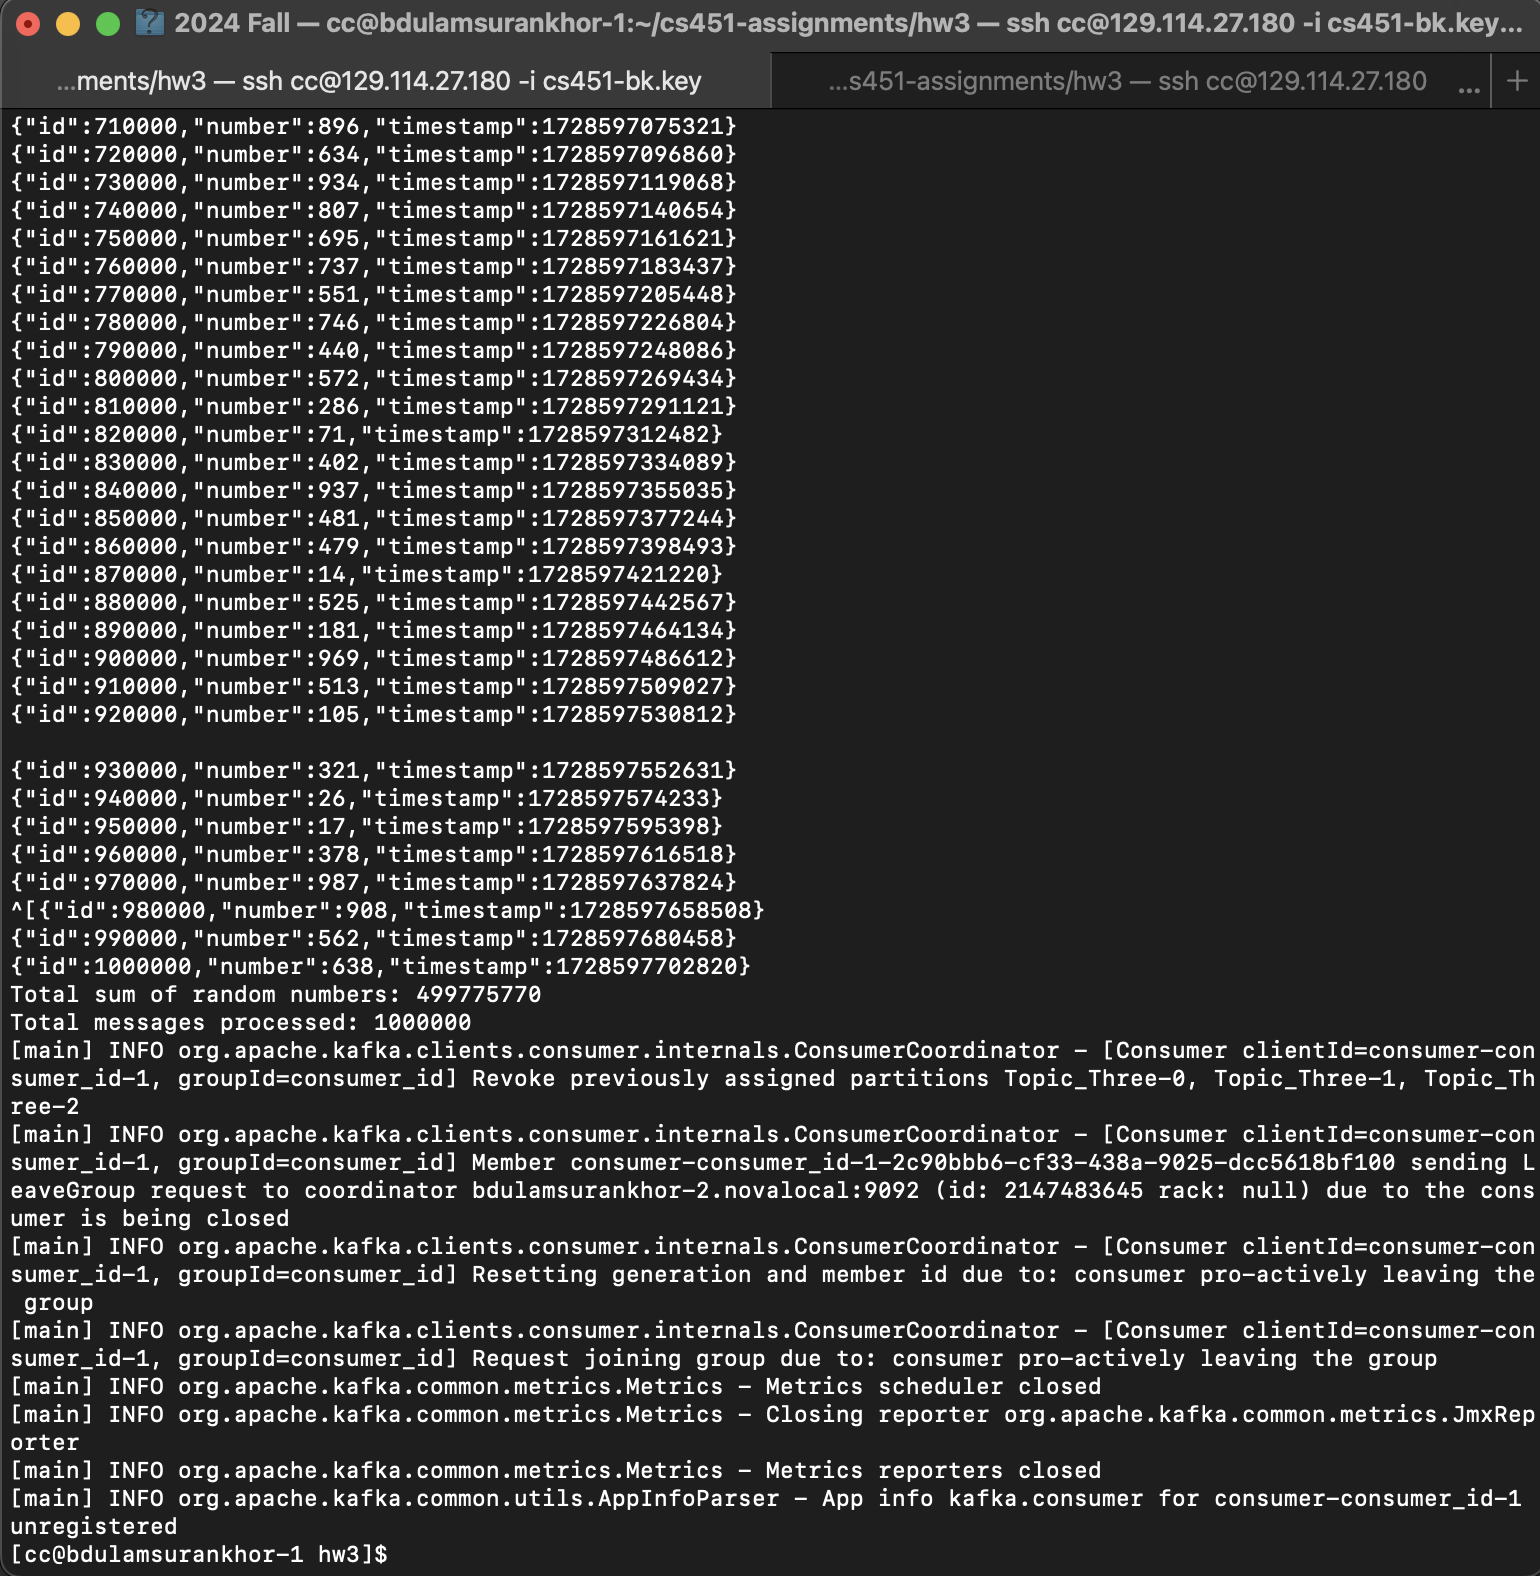
\includegraphics[width=1\textwidth]{image14.png}
        \caption{Topic\_Three consumer output.}
      \end{minipage}
      \begin{minipage}{0.45\textwidth}
        \centering
        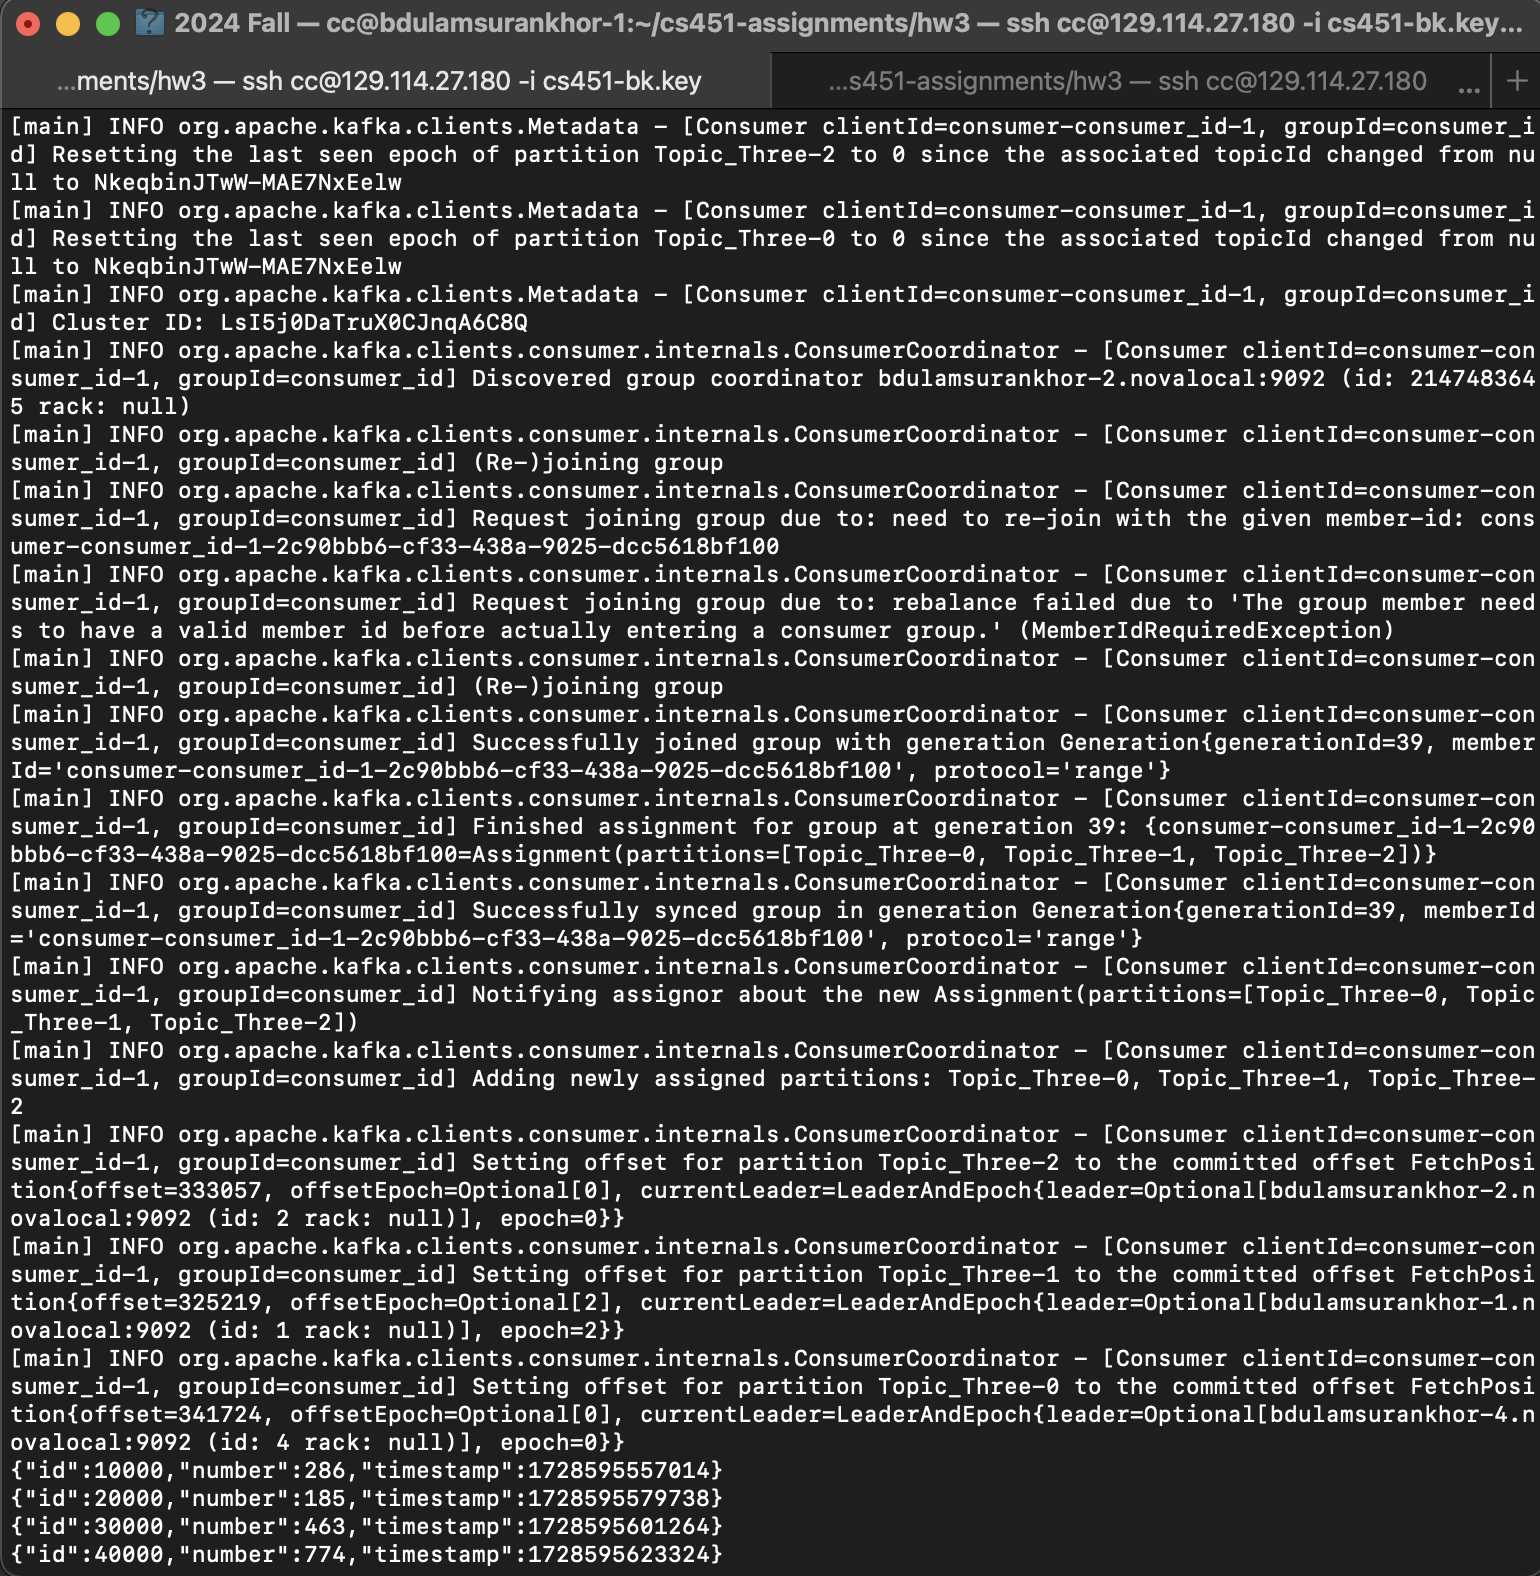
\includegraphics[width=1\textwidth]{image15.png}
        \caption{Topic\_Three consumer output.}
      \end{minipage}
    \end{figure}
    \item Topic\_Four
    \begin{figure}[H]
      \centering
      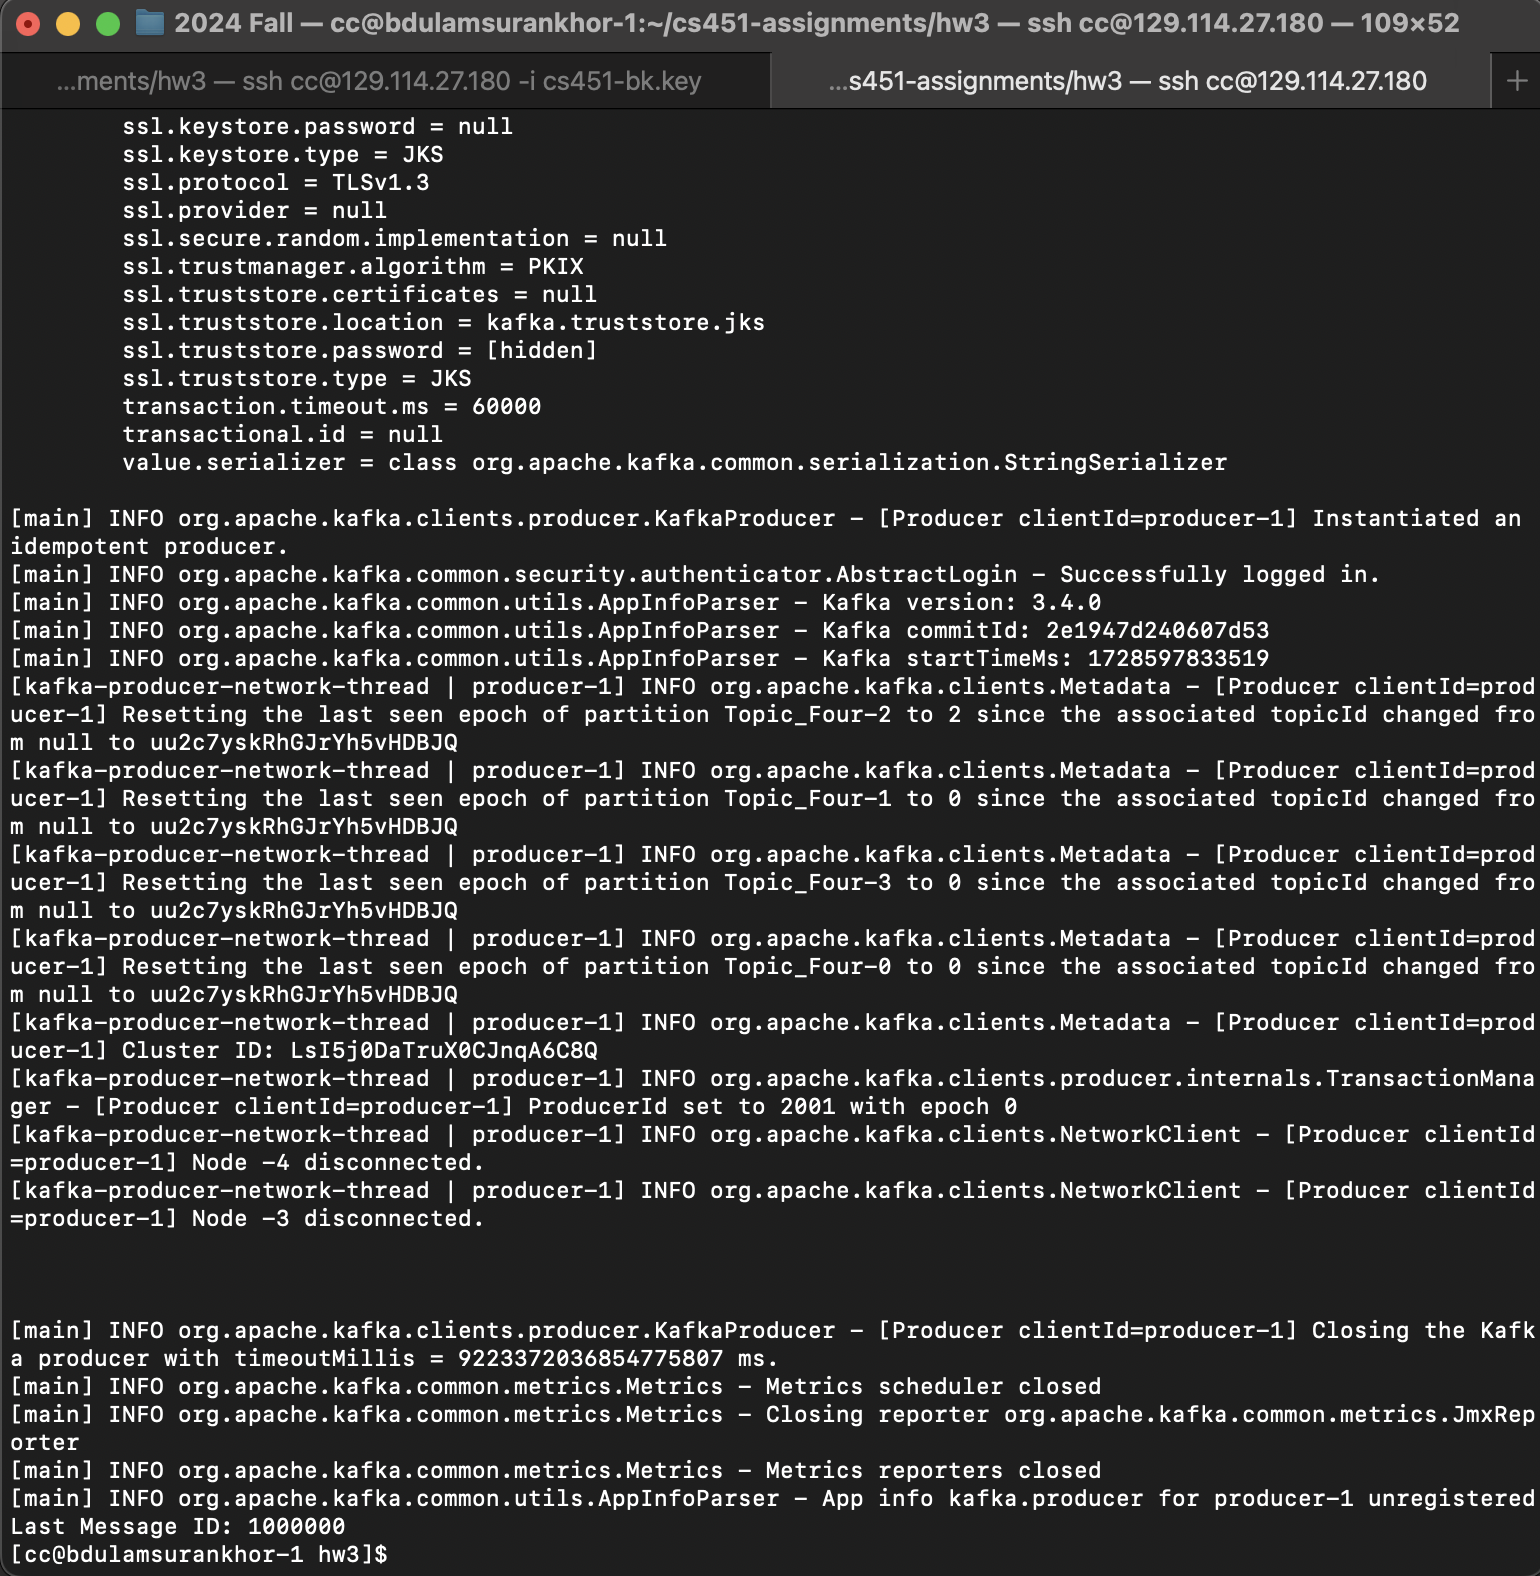
\includegraphics[width=0.6\textwidth]{image16.png}
      \caption{Topic\_Four producer output.}
    \end{figure}

    \begin{figure}[H]
      \centering
      \begin{minipage}{0.45\textwidth}
        \centering
        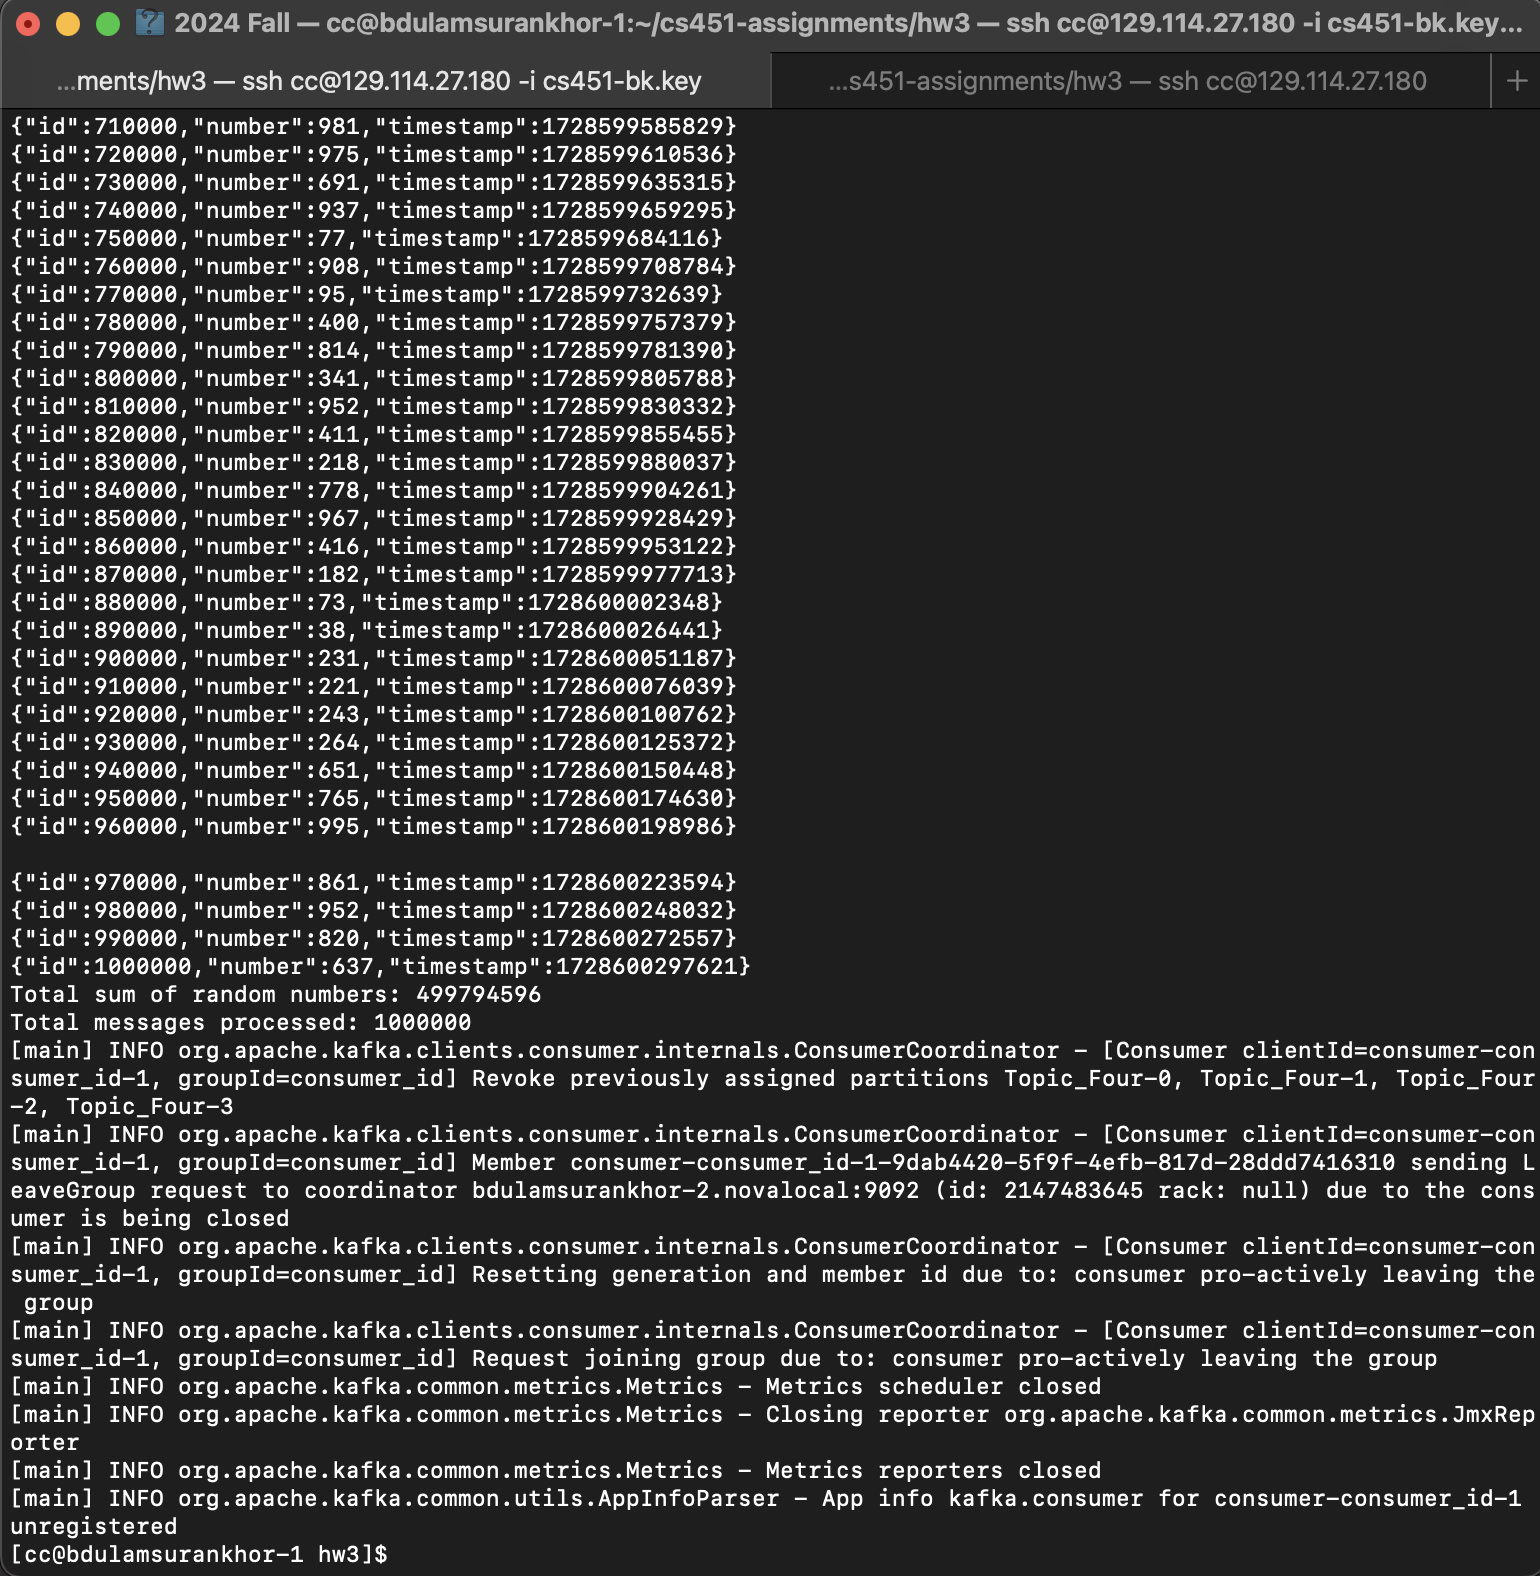
\includegraphics[width=1\textwidth]{image17.png}
        \caption{Topic\_Four consumer output.}
      \end{minipage}
      \begin{minipage}{0.45\textwidth}
        \centering
        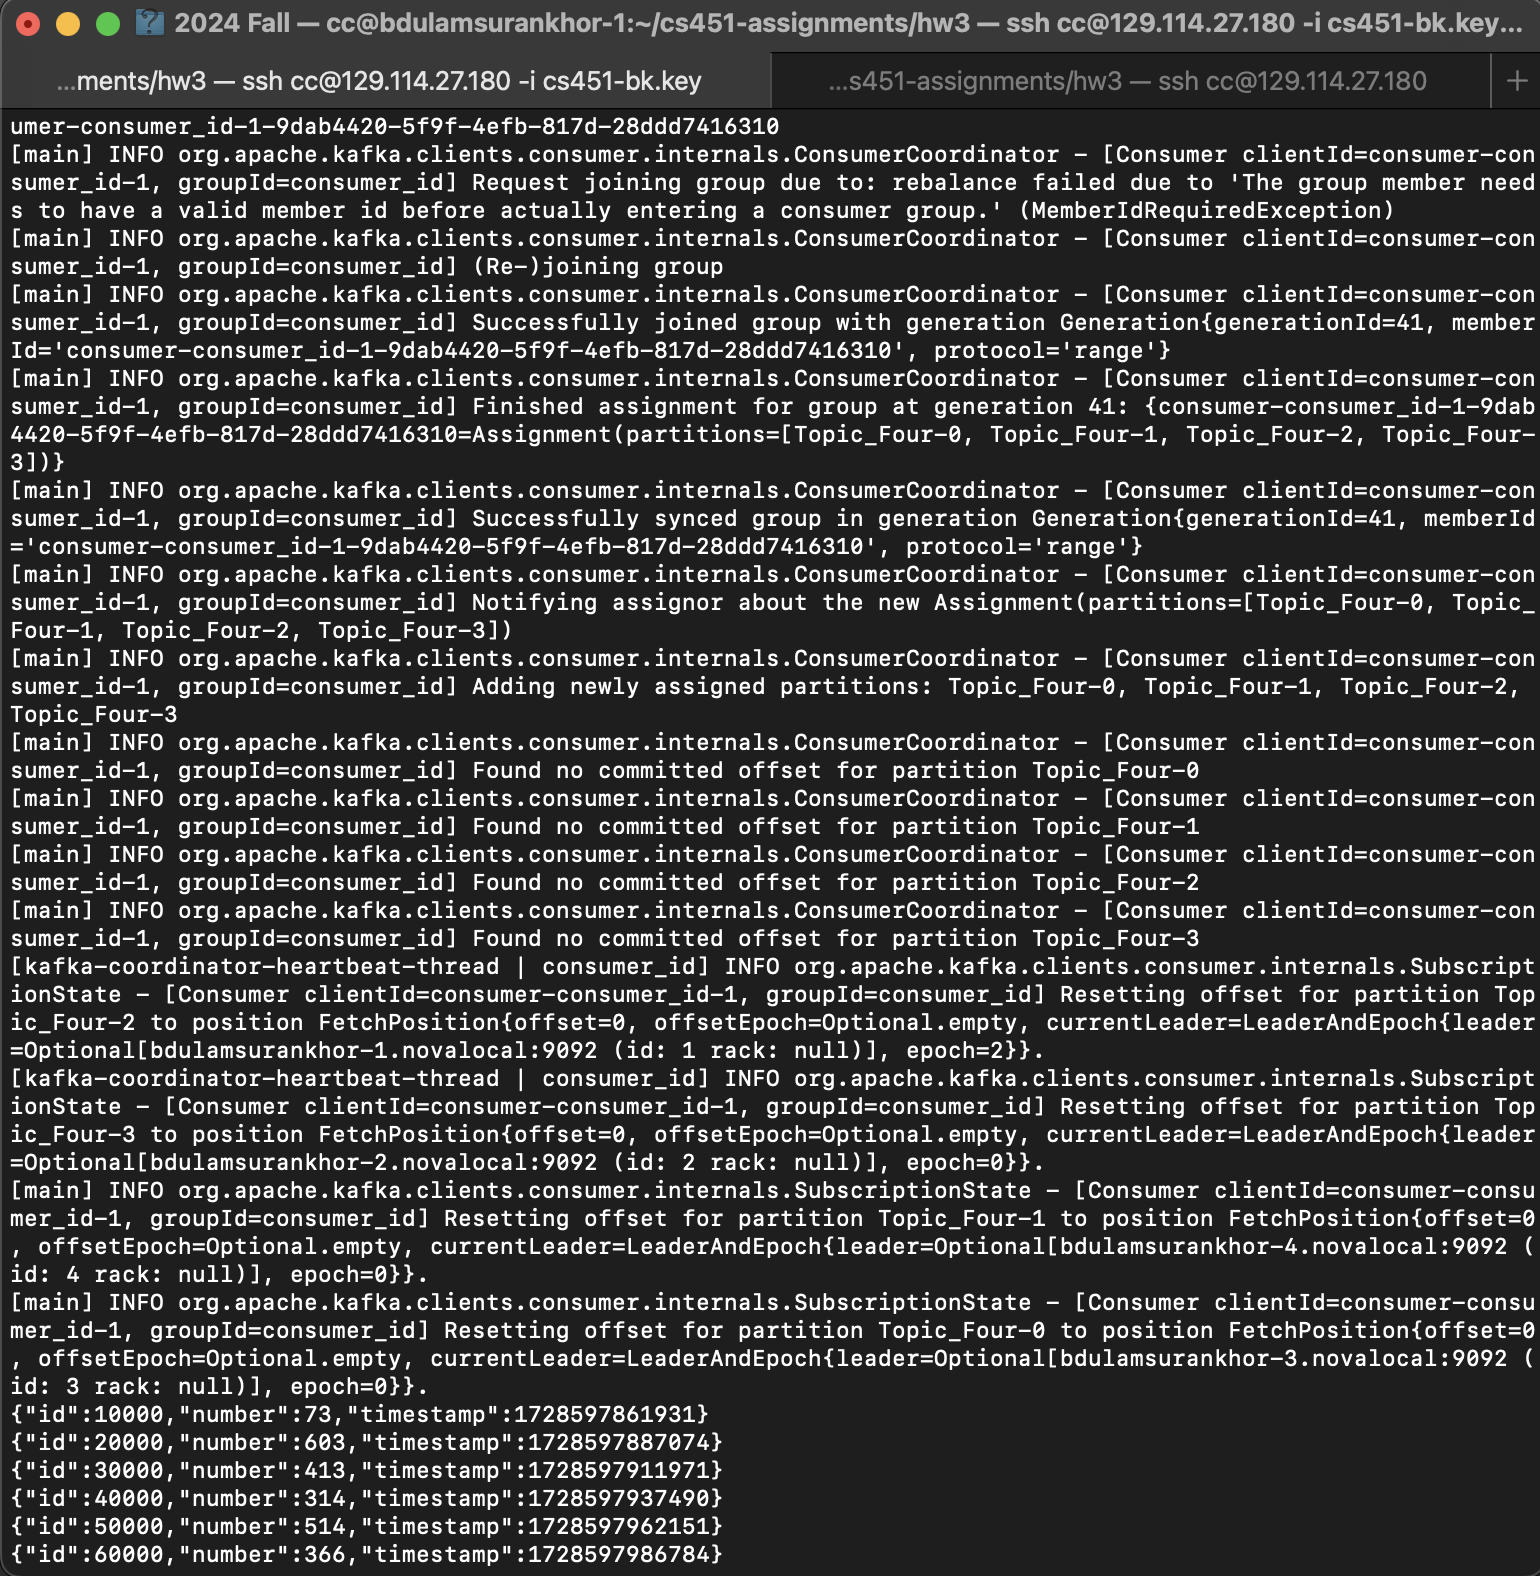
\includegraphics[width=1\textwidth]{image18.png}
        \caption{Topic\_Four consumer output.}
      \end{minipage}
    \end{figure}

    \item Retaking screenshot at 17.d after loading messages.
    \begin{figure}[H]
      \centering
      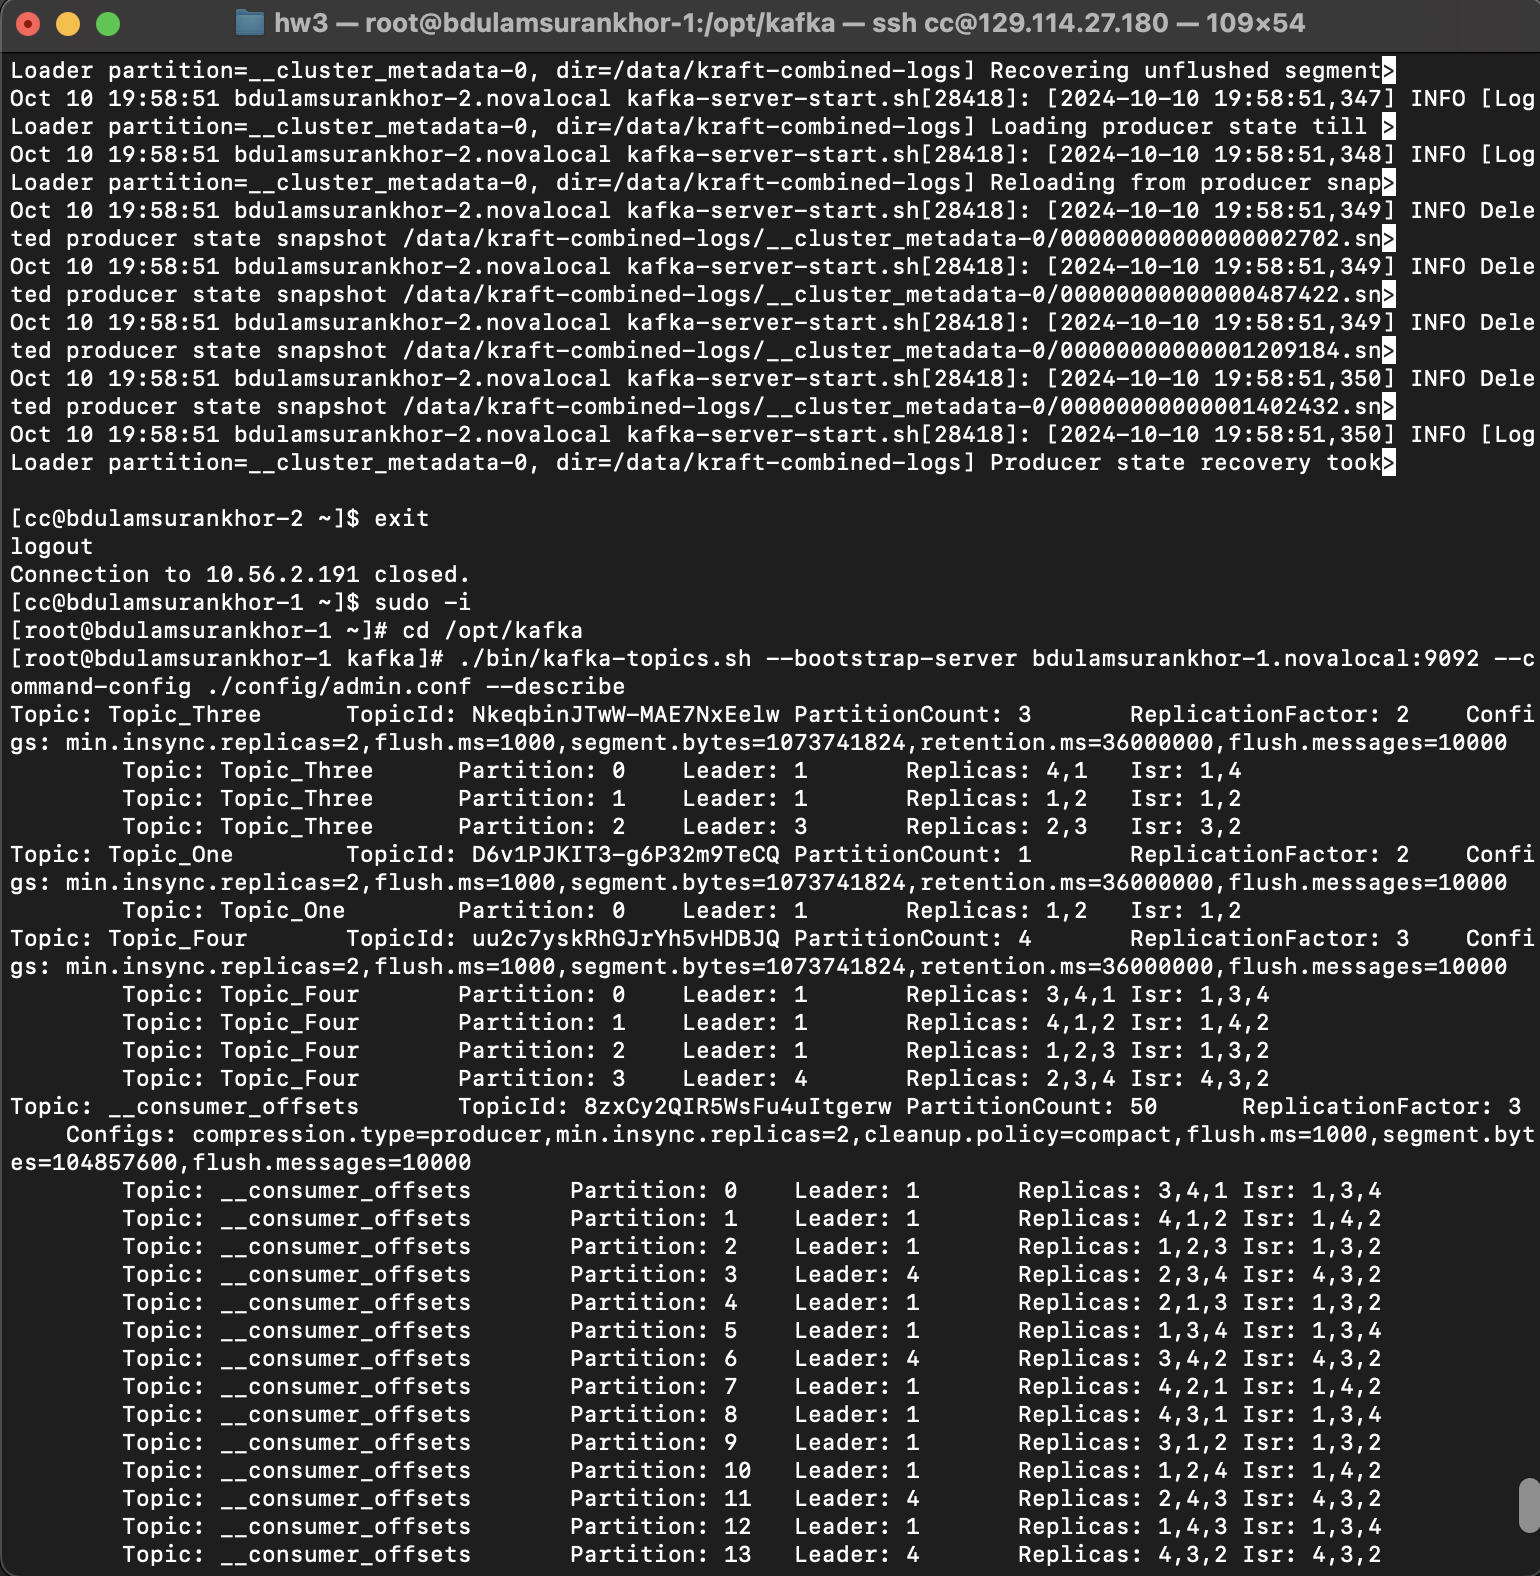
\includegraphics[width=0.6\textwidth]{image9.png}
      \caption{Retaking screenshot at 17.d after loading messages.}
    \end{figure}
  \end{enumerate}
\end{enumerate}

\end{document}